\noindent

%%%%%%%%%% CÂU 1 %%%%%%%%%%
{\normalcolor{\textbf{CÂU I. (4.0 điểm)}}}
\setcounter{equation}{0}


Cho một sợi dây thép cứng, nhẵn được uốn thành đa giác lồi $N$ cạnh có chiều dài các cạnh là $l_1, l_2,..., l_N$ và mặt bàn nhẵn nằm ngang có hình dạng giống hệt đa giác ở trên.
\begin{enumerate}[label=(\alph*)]
\item Ta uốn sợi dây thành đa giác đều ($l_1=l_2=...=l_N=l$). Giả sử rằng ta có $N$ ròng rọc rất nhỏ và rất nhẹ luồn vào từng cạnh của đa giác, sau đó buộc $N$ sợi dây nhẹ, không dãn sao cho một đầu được nối vào quả nặng $M$, đầu còn lại được nối vào những khối lượng bằng nhau có khối lượng $m$. Đặt khối lượng $M$ lên bàn và vắt mỗi sợi dây lên các ròng rọc có chỉ số các cạnh tương ứng (như hình vẽ bên dưới). Xét trong vùng mà mỗi cạnh của đa giác chỉ chứa một ròng rọc, hãy xác định các vị trí cân bằng trong khu vực này. Vẽ hình chỉ ra vị trí cân bằng cho trường hợp $N=5$ và $N=6$.

\begin{figure}[!h]
    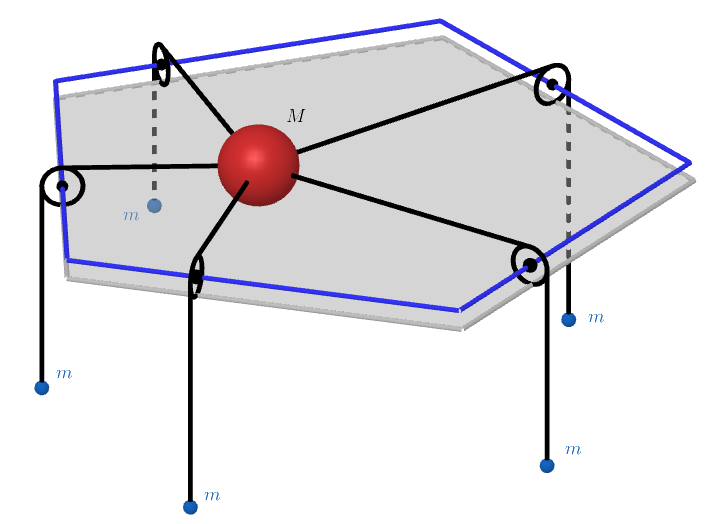
\includegraphics[width=0.5\linewidth]{Problem_1/Figs_P1/Figs_P1.png}
    \centering
    \label{fig:P1_01}
    \caption{}
\end{figure}
\item Xét trường hợp $N = 3$ (nói cách khác là cuốn sợi dây thành hình tam giác có cạnh $l_1, l_2, l_3$), sau đó luồn 3 hạt cườm rất nhẹ vào mỗi cạnh, mỗi hạt cườm lại có một lò xo có độ dài tự nhiên rất nhỏ (coi bằng 0) có độ cứng $k_1, k_2, k_3$ và một đầu của mỗi lò xo được gắn vào khối lượng $M$ (như hình ở dưới). Đặt vật $M$ trên bàn. Xác định vị trí cân bằng trong các trường hợp:
    \begin{enumerate}[label=(\roman*)]
    \item Độ dài các cạnh của tam giác và các độ cứng của lò xo thỏa mãn: $l_1:l_2:l_3=k_1:k_2:k_3$.
    \item Các độ cứng của lò xo bằng nhau và bằng $k$.
    \end{enumerate}
\begin{figure}[H]
    \centering
    % Gradient Info
  
\tikzset {_2c9ddldf2/.code = {\pgfsetadditionalshadetransform{ \pgftransformshift{\pgfpoint{89.1 bp } { -128.7 bp }  }  \pgftransformscale{1.32 }  }}}
\pgfdeclareradialshading{_8o830cp2v}{\pgfpoint{-72bp}{104bp}}{rgb(0bp)=(0.89,0.75,0.75);
rgb(0bp)=(0.89,0.75,0.75);
rgb(12.589285714285714bp)=(0.82,0.01,0.11);
rgb(400bp)=(0.82,0.01,0.11)}
\tikzset{every picture/.style={line width=0.75pt}} %set default line width to 0.75pt        

\begin{tikzpicture}[x=0.75pt,y=0.75pt,yscale=-1,xscale=1]
%uncomment if require: \path (0,462); %set diagram left start at 0, and has height of 462

%Shape: Triangle [id:dp3326541587702424] 
\draw  [color={rgb, 255:red, 74; green, 93; blue, 226 }  ,draw opacity=1 ][fill={rgb, 255:red, 128; green, 128; blue, 128 }  ,fill opacity=0.1 ][line width=3]  (179.94,26) -- (429,269.11) -- (50,269.11) -- cycle ;
%Shape: Inductor (Air Core) [id:dp6872930774599556] 
\draw  [line width=1.5]  (206.28,201.94) -- (206.02,213.91) .. controls (209.3,214.15) and (212.07,215.88) .. (213,218.25) .. controls (213.93,220.62) and (212.83,223.16) .. (210.23,224.64) .. controls (208.2,225.79) and (205.6,226.21) .. (203.09,225.82) .. controls (202.11,225.8) and (201.33,225.18) .. (201.35,224.45) .. controls (201.36,223.71) and (202.17,223.14) .. (203.15,223.16) .. controls (205.67,222.87) and (208.25,223.41) .. (210.23,224.64) .. controls (212.33,226.07) and (213.5,228.02) .. (213.45,230.03) .. controls (213.41,232.05) and (212.16,233.94) .. (209.99,235.28) .. controls (207.97,236.42) and (205.37,236.85) .. (202.86,236.45) .. controls (201.88,236.43) and (201.1,235.82) .. (201.12,235.08) .. controls (201.13,234.35) and (201.94,233.77) .. (202.92,233.79) .. controls (205.44,233.51) and (208.02,234.05) .. (209.99,235.28) .. controls (212.1,236.71) and (213.26,238.66) .. (213.22,240.67) .. controls (213.18,242.68) and (211.93,244.58) .. (209.76,245.91) .. controls (207.73,247.06) and (205.14,247.49) .. (202.63,247.09) .. controls (201.65,247.07) and (200.87,246.45) .. (200.88,245.72) .. controls (200.9,244.99) and (201.71,244.41) .. (202.69,244.43) .. controls (205.21,244.14) and (207.79,244.68) .. (209.76,245.91) .. controls (212.3,247.51) and (213.28,250.09) .. (212.25,252.42) .. controls (211.22,254.75) and (208.38,256.35) .. (205.09,256.45) -- (204.83,268.42) ;
%Shape: Inductor (Air Core) [id:dp16634280228018206] 
\draw  [line width=1.5]  (110.6,158.34) -- (126.29,165.64) .. controls (128.31,161.89) and (132.02,159.61) .. (135.64,159.89) .. controls (139.25,160.17) and (142.04,162.96) .. (142.66,166.91) .. controls (143.12,169.99) and (142.34,173.32) .. (140.52,176.06) .. controls (139.99,177.21) and (138.77,177.79) .. (137.81,177.34) .. controls (136.85,176.89) and (136.5,175.59) .. (137.04,174.44) .. controls (137.96,171.28) and (140.01,168.54) .. (142.66,166.91) .. controls (145.63,165.25) and (148.82,165.01) .. (151.46,166.23) .. controls (154.09,167.46) and (155.96,170.05) .. (156.6,173.4) .. controls (157.06,176.48) and (156.29,179.81) .. (154.46,182.55) .. controls (153.93,183.7) and (152.71,184.27) .. (151.75,183.83) .. controls (150.79,183.38) and (150.44,182.08) .. (150.98,180.93) .. controls (151.9,177.77) and (153.95,175.03) .. (156.6,173.4) .. controls (159.58,171.74) and (162.76,171.49) .. (165.4,172.72) .. controls (168.04,173.95) and (169.9,176.54) .. (170.54,179.89) .. controls (171.01,182.96) and (170.23,186.3) .. (168.41,189.04) .. controls (167.87,190.19) and (166.66,190.76) .. (165.69,190.31) .. controls (164.73,189.86) and (164.39,188.57) .. (164.92,187.42) .. controls (165.85,184.26) and (167.89,181.51) .. (170.54,179.89) .. controls (173.97,177.81) and (177.89,178.15) .. (180.44,180.74) .. controls (182.98,183.32) and (183.63,187.63) .. (182.06,191.59) -- (197.75,198.88) ;
%Shape: Inductor (Air Core) [id:dp3092264128133372] 
\draw  [line width=1.5]  (206.35,197.88) -- (221.06,185.93) .. controls (218.69,182.58) and (218.53,178.21) .. (220.65,174.91) .. controls (222.77,171.61) and (226.73,170.06) .. (230.65,171.01) .. controls (233.68,171.76) and (236.31,173.78) .. (237.87,176.55) .. controls (238.64,177.5) and (238.53,178.86) .. (237.63,179.6) .. controls (236.72,180.33) and (235.37,180.16) .. (234.6,179.21) .. controls (232.2,177.12) and (230.76,174.13) .. (230.65,171.01) .. controls (230.67,167.56) and (232.08,164.47) .. (234.56,162.46) .. controls (237.03,160.45) and (240.35,159.7) .. (243.72,160.38) .. controls (246.76,161.13) and (249.39,163.15) .. (250.94,165.93) .. controls (251.71,166.88) and (251.61,168.24) .. (250.7,168.97) .. controls (249.8,169.71) and (248.44,169.53) .. (247.67,168.58) .. controls (245.28,166.49) and (243.84,163.5) .. (243.72,160.38) .. controls (243.75,156.94) and (245.16,153.85) .. (247.64,151.84) .. controls (250.11,149.82) and (253.43,149.07) .. (256.8,149.76) .. controls (259.84,150.51) and (262.47,152.53) .. (264.02,155.3) .. controls (264.79,156.25) and (264.68,157.62) .. (263.78,158.35) .. controls (262.88,159.08) and (261.52,158.91) .. (260.75,157.96) .. controls (258.36,155.87) and (256.92,152.88) .. (256.8,149.76) .. controls (256.68,145.73) and (259.01,142.17) .. (262.67,140.77) .. controls (266.33,139.37) and (270.58,140.42) .. (273.37,143.43) -- (288.08,131.48) ;
%Flowchart: Delay [id:dp8143670880210933] 
\draw  [fill={rgb, 255:red, 0; green, 0; blue, 0 }  ,fill opacity=1 ] (109.35,153.2) -- (112.55,155.15) .. controls (114.31,156.22) and (114.87,158.52) .. (113.8,160.28) .. controls (112.73,162.05) and (110.43,162.61) .. (108.66,161.54) -- (105.47,159.59) -- cycle ;
%Flowchart: Delay [id:dp9198941962672681] 
\draw  [fill={rgb, 255:red, 0; green, 0; blue, 0 }  ,fill opacity=1 ] (200.88,271.94) -- (201.1,268.2) .. controls (201.22,266.14) and (202.99,264.57) .. (205.05,264.69) .. controls (207.11,264.81) and (208.68,266.58) .. (208.56,268.64) -- (208.35,272.37) -- cycle ;
%Flowchart: Delay [id:dp3222573149762976] 
\draw  [fill={rgb, 255:red, 0; green, 0; blue, 0 }  ,fill opacity=1 ] (293.37,131.19) -- (290.87,133.97) .. controls (289.49,135.51) and (287.12,135.64) .. (285.59,134.26) .. controls (284.05,132.88) and (283.92,130.51) .. (285.3,128.98) -- (287.8,126.19) -- cycle ;
%Flowchart: Connector [id:dp4674995309000146] 
\path  [shading=_8o830cp2v,_2c9ddldf2] (196.75,197.88) .. controls (196.75,192.58) and (201.05,188.29) .. (206.35,188.29) .. controls (211.64,188.29) and (215.94,192.58) .. (215.94,197.88) .. controls (215.94,203.18) and (211.64,207.47) .. (206.35,207.47) .. controls (201.05,207.47) and (196.75,203.18) .. (196.75,197.88) -- cycle ; % for fading 
 \draw  [color={rgb, 255:red, 208; green, 2; blue, 27 }  ,draw opacity=1 ][line width=0.75]  (196.75,197.88) .. controls (196.75,192.58) and (201.05,188.29) .. (206.35,188.29) .. controls (211.64,188.29) and (215.94,192.58) .. (215.94,197.88) .. controls (215.94,203.18) and (211.64,207.47) .. (206.35,207.47) .. controls (201.05,207.47) and (196.75,203.18) .. (196.75,197.88) -- cycle ; % for border 


% Text Node
\draw (230.7,278.69) node [anchor=north west][inner sep=0.75pt]    {$l_{1}$};
% Text Node
\draw (318.07,126.28) node [anchor=north west][inner sep=0.75pt]    {$l_{2}$};
% Text Node
\draw (86.23,124.46) node [anchor=north west][inner sep=0.75pt]    {$l_{3}$};
% Text Node
\draw (214.79,226.02) node [anchor=north west][inner sep=0.75pt]    {$k_{1}$};
% Text Node
\draw (222.27,133.76) node [anchor=north west][inner sep=0.75pt]    {$k_{2}$};
% Text Node
\draw (142.48,142.07) node [anchor=north west][inner sep=0.75pt]    {$k_{3}$};
% Text Node
\draw (217.94,201.28) node [anchor=north west][inner sep=0.75pt]    {$M$};
\end{tikzpicture}
\centering
\caption{}
\label{fig:P1_02}
\end{figure}
\end{enumerate}

Gợi ý: Có thể sử dụng định lý con nhím cho đa giác $N$ cạnh, tức là: 
\begin{equation}
l_1\vec{\hat{n}_1}+l_2\vec{\hat{n}_2}+...+l_N\vec{\hat{n}_N}=\vec{0}.
\end{equation}
Trong đó $\vec{\hat{n}_i}$ là vector đơn vị pháp tuyến với cạnh thứ $i$, hướng ra ngoài đa giác.

Hoặc có thể sử dụng việc vật đạt trạng thái cân bằng (bền) thì thế năng sẽ đạt giá trị cực tiểu.
\begin{center}
    \normalcolor{\textbf{Bài giải}}
\end{center}
\section{Cách giải 1: Cân bằng lực}
\begin{enumerate}[label=(\alph*)]
\item Do ròng rọc rất nhẹ và dây thép rất nhẵn nên lực tác dụng lên ròng rọc theo phương song song với cạnh bằng $0$, nói cách khác là dây có phương vuông góc với cạnh.

Khi hệ ở trạng thái cân bằng, ta dễ dàng thấy được lực căng do mỗi dây tác dụng lên $M$ là bằng nhau và có độ lớn là $T=mg$.

Áp dụng định lý con nhím cho đa giác $N$ cạnh, do $l_1=l_2=...=l_N=l$ nên phương trình đã cho trở thành:
\begin{equation}
\vec{\hat{n}_1}+\vec{\hat{n}_2}+...+\vec{\hat{n}_N}=\vec{0}.
\end{equation}

Nhân cả hai vế với $T$ và do $\vec{T_i}$ (vector lực căng dây tương ứng với ròng rọc ở cạnh thứ $i$) song song và cùng chiều với $\vec{\hat{n_i}}$ nên:
\begin{equation}
\vec{T_1} + \vec{T_2}+...+\vec{T_N}=\vec{0}.
\end{equation}
Hay là tổng hợp lực tác dụng lên $M$ bằng $0$ vậy nên vật $M$ ở trạng thái cân bằng tại mọi vị trí bên trong khu vực mà mỗi cạnh chỉ chứa một ròng rọc.

Ta có các vị trí cân bằng ứng với $N=5$ và $N=6$ (các vùng được tô xanh và hồng tương ứng) như hình vẽ sau:
\begin{figure}[H]
\scalebox{0.75}{
\definecolor{fuqqzz}{rgb}{0.9568627450980393,0,0.6}
\definecolor{qqqqff}{rgb}{0,0,1}
\definecolor{ttzzqq}{rgb}{0.2,0.6,0}
\definecolor{zzttqq}{rgb}{0.6,0.2,0}
\begin{tikzpicture}[line cap=round,line join=round,>=triangle 45,x=1cm,y=1cm]
\clip(-8.873415233529899,-3.7005639828456323) rectangle (14.615466183323264,9.59429794121481);
\fill[line width=2pt,color=zzttqq,fill=zzttqq,fill opacity=0.10000000149011612] (-5,0) -- (-2,0) -- (-1.0729490168751576,2.85316954888546) -- (-3.5,4.616525305762879) -- (-5.9270509831248415,2.853169548885461) -- cycle;
\fill[line width=2pt,color=ttzzqq,fill=ttzzqq,fill opacity=0.1] (2,0) -- (5,0) -- (6.5,2.598076211353316) -- (5,5.196152422706633) -- (2,5.196152422706634) -- (0.5,2.5980762113533187) -- cycle;
\fill[line width=2pt,color=qqqqff,fill=qqqqff,fill opacity=0.2] (-4.427050983124842,3.34054909323482) -- (-3.5,3.6417662170641605) -- (-2.5729490168751594,3.3405490932348205) -- (-2,2.551952425056118) -- (-2,1.5771933363574) -- (-2.572949016875158,0.7885966681786997) -- (-3.5,0.4873795443493592) -- (-4.427050983124842,0.7885966681787006) -- (-5,1.5771933363574013) -- (-5,2.55195242505612) -- cycle;
\fill[line width=2pt,color=fuqqzz,fill=fuqqzz,fill opacity=0.45] (3.5,4.330127018922194) -- (5,3.4641016151377544) -- (5,1.7320508075688759) -- (3.5,0.8660254037844383) -- (2,1.7320508075688772) -- (2,3.464101615137757) -- cycle;
\draw [line width=2pt,color=zzttqq] (-5,0)-- (-2,0);
\draw [line width=2pt,color=zzttqq] (-2,0)-- (-1.0729490168751576,2.85316954888546);
\draw [line width=2pt,color=zzttqq] (-1.0729490168751576,2.85316954888546)-- (-3.5,4.616525305762879);
\draw [line width=2pt,color=zzttqq] (-3.5,4.616525305762879)-- (-5.9270509831248415,2.853169548885461);
\draw [line width=2pt,color=zzttqq] (-5.9270509831248415,2.853169548885461)-- (-5,0);
\draw [line width=2pt,color=ttzzqq] (2,0)-- (5,0);
\draw [line width=2pt,color=ttzzqq] (5,0)-- (6.5,2.598076211353316);
\draw [line width=2pt,color=ttzzqq] (6.5,2.598076211353316)-- (5,5.196152422706633);
\draw [line width=2pt,color=ttzzqq] (5,5.196152422706633)-- (2,5.196152422706634);
\draw [line width=2pt,color=ttzzqq] (2,5.196152422706634)-- (0.5,2.5980762113533187);
\draw [line width=2pt,color=ttzzqq] (0.5,2.5980762113533187)-- (2,0);
\draw (3,-0.3) node[anchor=north west] {$N=6$};
\draw (-4,-0.3) node[anchor=north west] {$N=5$};
\end{tikzpicture}
}
\centering
\caption{}
\label{figs:S1_01}
\end{figure}
Ta vẽ các vị trí trên bằng cách từ một đỉnh ta hạ đường thẳng vuông góc với hai cạnh kề với đỉnh đó (do dây luôn vuông góc với cạnh và ta xác định vùng mà ròng rọc nằm trên cạnh đó bằng cách kẻ đường vuông góc với cạnh từ hai đầu mút của mỗi cạnh, khi đó không gian nằm giữa hai đường thẳng vừa kẻ là vùng mà ròng rọc vẫn nằm trên cạnh đó) ta dễ dàng tìm được khu vực mà vật $M$ sẽ cân bằng (Ngoài ra, ta có thể để ý rằng đối với $N$ lẻ thì khu vực đó có dạng $2N$ giác đều còn $N$ chẵn thì khu vực đó có dạng $N$ giác đều)
\item Ta cũng lập luận tương tự ý trên ta suy ra được rằng lò xo vuông góc với cạnh. Ta kí hiệu $d_1,d_2,d_3$ lần lượt là khoảng cách từ $M$ đến các cạnh có chiều dài $l_1,l_2,l_3$.

Sử dụng định lí con nhím cho tam giác:
\begin{equation}
l_1\vec{\hat{n}_1}+l_2\vec{\hat{n}_2}+l_3\vec{\hat{n}_3}=\vec{0}.
\end{equation}

Lực đàn hồi ứng với cạnh thứ $i$ hướng song song và cùng chiều với vector $\vec{\hat{n}_i}$. Theo định luật Hooke, ta có lực đàn hồi: $\vec{F_i}=k_id_i\vec{\hat{n}_i}$.

Từ các biếu thức trên, ta được:
\begin{equation}
\label{eq:S1_01}
\dfrac{l_1}{k_1d_1}k_1d_1\vec{\hat{n_1}}+\dfrac{l_2}{k_2d_2}k_2d_2\vec{\hat{n_2}}+\dfrac{l_3}{k_3d_3}k_3d_3\vec{\hat{n_3}}=\vec{0}.
\end{equation}

\begin{equation}
\Longrightarrow\dfrac{l_1}{k_1d_1}\vec{F_1}+\dfrac{l_2}{k_2d_2}\vec{F_2}+\dfrac{l_3}{k_3d_3}\vec{F_3}=\vec{0}.
\end{equation}

Để cân bằng lực, $\vec{F_1}+\vec{F_2}+\vec{F_3}=\vec{0}$:

\begin{equation}
\label{eq:S1_02}
\Longrightarrow \dfrac{l_1}{k_1d_1}=\dfrac{l_2}{k_2d_2}=\dfrac{l_3}{k_3d_3}.
\end{equation}
    \begin{enumerate}[label=(\roman*)]
    \item Trong trường hợp $l_1:l_2:l_3=k_1:k_2:k_3$, ta dễ dàng suy ra được $d_1=d_2=d_3$. Nói cách khác, điểm $M$ khi đó nằm cân bằng ở tâm đường tròn nội tiếp của tam giác.
    \item Trong trường hợp $k_1=k_2=k_3=k$, ta được: 
    \begin{equation}
    \label{eq:S1_03}
    \dfrac{l_1}{d_1}=\dfrac{l_2}{d_2}=\dfrac{l_3}{d_3}.
    \end{equation}
    Khi đó ta thấy được rằng điểm $M$ nằm cân bằng ở điểm Lemoine của tam giác như sau:

    Ta đặt các đỉnh của tam giác là $A,B,C$. Hình chiếu của $M$ lên $BC,CA,AB$ là $M_1,M_2,M_3$. Ta dựng phân giác góc $A$ và lấy điểm $M'$ đối xứng với $M$ qua đường phân giác. Gọi giao điểm của $AM'$ với $BC$ là $A'$ (xem hình vẽ bên dưới).

\begin{figure}[H]    
\centering
% Gradient Info
  
\tikzset {_90k2znmbz/.code = {\pgfsetadditionalshadetransform{ \pgftransformshift{\pgfpoint{89.1 bp } { -128.7 bp }  }  \pgftransformscale{1.32 }  }}}
\pgfdeclareradialshading{_t67nn9g7p}{\pgfpoint{-72bp}{104bp}}{rgb(0bp)=(0.89,0.75,0.75);
rgb(0bp)=(0.89,0.75,0.75);
rgb(12.589285714285714bp)=(0.82,0.01,0.11);
rgb(400bp)=(0.82,0.01,0.11)}
\tikzset{every picture/.style={line width=0.75pt}} %set default line width to 0.75pt        

\begin{tikzpicture}[x=0.75pt,y=0.75pt,yscale=-1,xscale=1]
%uncomment if require: \path (0,462); %set diagram left start at 0, and has height of 462

%Shape: Triangle [id:dp3326541587702424] 
\draw  [color={rgb, 255:red, 74; green, 93; blue, 226 }  ,draw opacity=1 ][fill={rgb, 255:red, 128; green, 128; blue, 128 }  ,fill opacity=0.1 ][line width=3]  (179.94,26) -- (429,269.11) -- (50,269.11) -- cycle ;
%Flowchart: Delay [id:dp8143670880210933] 
\draw  [fill={rgb, 255:red, 0; green, 0; blue, 0 }  ,fill opacity=1 ] (101.75,161.68) -- (105.21,163.09) .. controls (107.13,163.87) and (108.05,166.05) .. (107.27,167.97) .. controls (106.49,169.88) and (104.31,170.8) .. (102.39,170.02) -- (98.93,168.61) -- cycle ;
%Flowchart: Delay [id:dp9198941962672681] 
\draw  [fill={rgb, 255:red, 0; green, 0; blue, 0 }  ,fill opacity=1 ] (180.61,272.15) -- (180.83,268.42) .. controls (180.95,266.36) and (182.72,264.78) .. (184.78,264.9) .. controls (186.84,265.02) and (188.42,266.79) .. (188.3,268.86) -- (188.08,272.59) -- cycle ;
%Flowchart: Delay [id:dp3222573149762976] 
\draw  [fill={rgb, 255:red, 0; green, 0; blue, 0 }  ,fill opacity=1 ] (284.07,122.71) -- (281.57,125.5) .. controls (280.19,127.03) and (277.82,127.16) .. (276.29,125.78) .. controls (274.75,124.4) and (274.62,122.04) .. (276,120.5) -- (278.5,117.72) -- cycle ;
%Flowchart: Connector [id:dp4674995309000146] 
\path  [shading=_t67nn9g7p,_90k2znmbz] (176.49,198.1) .. controls (176.49,192.8) and (180.78,188.5) .. (186.08,188.5) .. controls (191.38,188.5) and (195.67,192.8) .. (195.67,198.1) .. controls (195.67,203.39) and (191.38,207.69) .. (186.08,207.69) .. controls (180.78,207.69) and (176.49,203.39) .. (176.49,198.1) -- cycle ; % for fading 
 \draw  [color={rgb, 255:red, 208; green, 2; blue, 27 }  ,draw opacity=1 ][line width=0.75]  (176.49,198.1) .. controls (176.49,192.8) and (180.78,188.5) .. (186.08,188.5) .. controls (191.38,188.5) and (195.67,192.8) .. (195.67,198.1) .. controls (195.67,203.39) and (191.38,207.69) .. (186.08,207.69) .. controls (180.78,207.69) and (176.49,203.39) .. (176.49,198.1) -- cycle ; % for border 

%Straight Lines [id:da2866658385087255] 
\draw    (179.94,26) -- (241,268.5) ;
%Straight Lines [id:da04794658376262384] 
\draw  [dash pattern={on 0.84pt off 2.51pt}]  (107,168.5) -- (186.08,198.1) ;
%Straight Lines [id:da19647849123319838] 
\draw  [dash pattern={on 0.84pt off 2.51pt}]  (186.08,198.1) -- (184.56,268.64) ;
%Straight Lines [id:da7185203893957963] 
\draw  [dash pattern={on 0.84pt off 2.51pt}]  (186.08,198.1) -- (276,120.5) ;
%Straight Lines [id:da4577311492825563] 
\draw  [dash pattern={on 3.75pt off 3pt on 7.5pt off 1.5pt}]  (179.94,26) -- (212,268.5) ;
%Straight Lines [id:da048770005146599904] 
\draw    (179.94,26) -- (186.08,198.1) ;
%Straight Lines [id:da004397076478948825] 
\draw    (50,269.11) -- (223,195.5) ;
%Straight Lines [id:da0889957519920831] 
\draw    (223,195.5) -- (429,269.11) ;

% Text Node
\draw (218.7,283.69) node [anchor=north west][inner sep=0.75pt]    {$l_{1}$};
% Text Node
\draw (325.07,140.28) node [anchor=north west][inner sep=0.75pt]    {$l_{2}$};
% Text Node
\draw (67.23,168.46) node [anchor=north west][inner sep=0.75pt]    {$l_{3}$};
% Text Node
\draw (174.49,201.5) node [anchor=north east] [inner sep=0.75pt]    {$M$};
% Text Node
\draw (177.94,22.6) node [anchor=south east] [inner sep=0.75pt]    {$A$};
% Text Node
\draw (48,272.51) node [anchor=north east] [inner sep=0.75pt]    {$B$};
% Text Node
\draw (431,272.51) node [anchor=north west][inner sep=0.75pt]    {$C$};
% Text Node
\draw (182.61,275.55) node [anchor=north west][inner sep=0.75pt]    {$M_{1}$};
% Text Node
\draw (280.78,119.6) node [anchor=south west] [inner sep=0.75pt]    {$M_{2}$};
% Text Node
\draw (100.55,158.02) node [anchor=south east] [inner sep=0.75pt]    {$M_{3}$};
% Text Node
\draw (243,271.9) node [anchor=north west][inner sep=0.75pt]    {$A'$};
% Text Node
\draw (225,192.1) node [anchor=south west] [inner sep=0.75pt]    {$M'$};


\end{tikzpicture}
\caption{}
\label{figs:S1_02}
\end{figure}

    Do đối xứng qua phân giác góc $A$ nên $M'$ khoảng cách đến $AB$ là $d_2$, cách $AC$ là $d_3$. Từ điều kiện ở trên ta được $d_3l_2=d_2l_3$, hay diện tích các tam giác sau bằng nhau: 
    \begin{equation}
    A_{AM'B}=A_{AM'C}
    \end{equation}
    \begin{equation}
    \Longrightarrow 
    \dfrac{1}{2}l_3AM'\sin{\widehat{BAA'}}=\dfrac{1}{2}l_2AM'\sin{\widehat{CAA'}}.
    \end{equation}
    \begin{equation}
    \Longrightarrow l_3AA'\sin{\widehat{BAA'}}=l_2AA'\sin{\widehat{CAA'}}.
    \end{equation}
    \begin{equation}
    \Longrightarrow A_{AA'B}=A_{AA'C}.
    \end{equation}
    \begin{equation}
    \Longrightarrow A'B=A'C=\dfrac{l_1}{2}.
    \end{equation}
    Điều đó chứng tỏ rằng $A'$ là trung điểm $BC$, nói cách khác $AA'$ là đường trung tuyến ứng với $A$ của tam giác $ABC$ và $AM$ là đường đối trung tương ứng với đỉnh $A$. Tương tự, ta sẽ suy ra được rằng điểm $M$ là giao điểm của ba đường đối trung hay chính là điểm Lemoine.

    
    \end{enumerate}
\end{enumerate}

\textbf{Phổ điểm}
    \begin{center}
    \begin{tabular}{|c|p{8cm}|c|}
    \hline
    \multicolumn{1}{|l|}{Phần} & Nội dung & Điểm thành phần \\ 
    \hline
\multirow{4}{*}{(a)} & Chỉ ra rằng dây vuông góc với các cạnh.
                     & 0.25
                     \\
                     \cline{2-3}
                     & Chỉ ra tất cả các vị trí cân bằng.      
                     & 0.5           
                     \\ 
                     \cline{2-3}
                     & Vẽ hình trường hợp $N = 5$, $N = 6$.        
                     & 0.25           
                     \\
                     \cline{2-3}
                     \hline  
\multirow{4}{*}{(b)} & Chỉ ra rằng lò xo vuông góc với cạnh tam giác.                                       & 0.25             
                     \\
                     \cline{2-3}
                     & Lập luận được biểu thức \eqref{eq:S1_01}. 
                     & 0.25
                     \\
                     \cline{2-3}
                     & Ra được biểu thức \eqref{eq:S1_02}. 
                     & 1.0
                     \\
                     \hline
\multirow{1}{*}{(b)(i)}& Chỉ ra rằng M cân bằng ở tâm đường tròn nội tiếp của tam giác.
                     & 0.5    
                     \\
                     \hline
\multirow{3}{*}{(b)(ii)}
                     &Ra được biểu thức \eqref{eq:S1_03}.     
                     & 0.5
                     \\
                     \cline{2-3}
                     & Chứng minh được M cân bằng ở điểm Lemoine.  
                     & 0.5
                     \\ \hline
                         


    \end{tabular}
    \end{center}

\section{Cách giải 2: Cực tiểu thế năng}
\begin{enumerate}[label=(\alph*)]
\item Ta cũng lập luận như cách 1 để suy ra rằng dây vuông góc với các cạnh. Để cân bằng, tức là thế năng của hệ phải cực tiểu, mà thế năng của hệ là tổng của các thế năng trọng trường $V_i$, với $V_i=-mgh_i$ (ta bỏ qua hằng số vì nó không quan trọng ở đây) với $h_i$ là độ cao của mặt bàn so với khối lượng $m$ ở cạnh thứ $i$ hay chính là chiều dài phần lơ lửng của dây thứ $i$. Do chiều dài từng dây không đổi nên thế năng là $V=\sum mgd_i$ với $d_i$ là chiều dài dây thứ $i$ còn lại, cũng chính là khoảng cách từ $M$ đến cạnh thứ $i$. Tức là thế năng tỉ lệ với $\sum d_i$. Tuy nhiên, tổng này không đổi vì khi ta nhân thêm chiều dài mỗi cạnh $l$, ta thu được diện tích của đa giác. Vậy nên tại mọi vị trí mà mỗi cạnh chỉ chứa một ròng rọc, vật $M$ luôn cân bằng.

Những phần còn lại của ý này giải y hệt cách 1.
\item Cũng tương tự cách 1, ta suy ra được lò xo vuông góc với từng cạnh của tam giác. Để cân bằng, tức là thế năng của hệ phải cực tiểu, mà thế năng của hệ là tổng của các thế năng đàn hồi $V_i$, với $V_i=\dfrac{1}{2} k_id_i^2$ (ta có thể vẽ đồ thị của lực đàn hồi $F_i=-k_ix$ theo $x$ và tính công để đi từ vị trí $x=d_i$ về $0$, để làm điều này ta tính diện tích tam giác vuông và suy ra $V_i=\dfrac{1}{2} (0-k_id_i)(0-d_i)$ và thu được biểu thức ở trên). Khi đó thế năng của cả hệ là:
\begin{equation}
V=\dfrac{1}{2}(k_1d_1^2+k_2d_2^2+k_3d_3^2).
\end{equation}

Diện tích của tam giác là hằng số: \begin{equation}
A=\dfrac{1}{2}(d_1l_1+d_2l_2+d_3l_3).
\end{equation}

Ta có 
\begin{equation}
V \propto (k_1d_1^2+k_2d_2^2+k_3d_3^2) \propto (k_1d_1^2+k_2d_2^2+k_3d_3^2)(\dfrac{l_1^2}{k_1}+\dfrac{l_2^2}{k_2}+\dfrac{l_3^2}{k_3}).
\end{equation}

Sử dụng bất đẳng thức Cauchy-Schwarz, ta được:
\begin{equation}(k_1d_1^2+k_2d_2^2+k_3d_3^2)(\dfrac{l_1^2}{k_1}+\dfrac{l_2^2}{k_2}+\dfrac{l_3^2}{k_3})\ge(l_1d_1+l_2d_2+l_3d_3)^2\propto A^2\ = const.
\end{equation}

Đẳng thức xảy ra khi và chỉ khi: 
\begin{equation}
\dfrac{l_1}{k_1d_1}=\dfrac{l_2}{k_2d_2}=\dfrac{l_3}{k_3d_3}.
\end{equation}

Phần còn lại y hệt như cách 1. Nhận xét:

\begin{enumerate}[label=(\roman*)]
    \item Từ hai cách giải vừa rồi ta không những thu được kết quả quen thuộc là $l_1\vec{d_1}+l_2\vec{d_2}+l_3\vec{d_3}=\vec{0}$ mà còn thu được kết quả là tâm đường tròn nội tiếp khiến cho biểu thức $l_1d_1^2+l_2d_2^2+l_3d_3^2$ cực tiểu.
    \item Hai cách giải trên giúp ta thu được hai tính chất của điểm Lemoine là $\vec{d_1}+\vec{d_2}+\vec{d_1}=\vec{0}$ và điểm Lemoine khiến cho tổng bình phương khoảng cách từ điểm đó đến ba cạnh cực tiểu.
\end{enumerate}
\end{enumerate}

\begin{flushright}
    (biên soạn bởi DMQ và carina)
\end{flushright}
\newpage

%%%%%%%%%% CÂU 2 %%%%%%%%%%
{\normalcolor{\textbf{CÂU II. (4.0 điểm)}}\vspace{1.5mm}}
\setcounter{equation}{0}


Nguyên lý Scheimpflug được đặt theo tên của kỹ sư người Áo Theodor Scheimpflug, mô tả cách một mặt phẳng tiêu cự có thể nghiêng để mở rộng vùng ảnh rõ nét trong nhiếp ảnh và quang học. 

Cụ thể, nguyên lý Scheimpflug phát biểu rằng khi mặt phẳng vật, mặt phẳng thấu kính và mặt phẳng ảnh (cảm biến hoặc phim) không song song mà giao nhau tại một đường thẳng chung, thì toàn bộ mặt phẳng vật nghiêng này vẫn có thể được lấy nét rõ ràng. 
\begin{enumerate}[label=(\alph*)]
\item Chứng minh nguyên lý Scheimpflug
\item Chứng minh rằng mặt phẳng tiêu cự quay quanh một trục đi qua điểm G khi ta nghiêng thấu kính \\
\begin{figure}[H]
    \centering
    \tikzset{every picture/.style={line width=0.75pt}} %set default line width to 0.75pt        

\begin{tikzpicture}[x=0.75pt,y=0.75pt,yscale=-1,xscale=1]
%uncomment if require: \path (0,424); %set diagram left start at 0, and has height of 424

%Straight Lines [id:da17793481393532118] 
\draw    (100,106) -- (411,330) ;
%Straight Lines [id:da4232639599589497] 
\draw    (411,88) -- (411,330) ;
%Straight Lines [id:da11938100176501354] 
\draw    (331,52) -- (411,330) ;
%Straight Lines [id:da838504233570497] 
\draw [color={rgb, 255:red, 215; green, 208; blue, 208 }  ,draw opacity=1 ]   (108,111) -- (411,209) ;
%Straight Lines [id:da49314275647124217] 
\draw [color={rgb, 255:red, 215; green, 208; blue, 208 }  ,draw opacity=1 ]   (255.5,218) -- (411,189) ;
%Straight Lines [id:da48246879037954804] 
\draw [color={rgb, 255:red, 14; green, 39; blue, 252 }  ,draw opacity=1 ]   (372,49) -- (373,360) ;
%Curve Lines [id:da20103497237081303] 
\draw [color={rgb, 255:red, 14; green, 39; blue, 252 }  ,draw opacity=1 ]   (195,174) .. controls (223.86,123.25) and (302.21,77.46) .. (370.96,92.76) ;
\draw [shift={(372,93)}, rotate = 193.06] [color={rgb, 255:red, 14; green, 39; blue, 252 }  ,draw opacity=1 ][line width=0.75]    (10.93,-3.29) .. controls (6.95,-1.4) and (3.31,-0.3) .. (0,0) .. controls (3.31,0.3) and (6.95,1.4) .. (10.93,3.29)   ;
%Curve Lines [id:da766499281537382] 
\draw [color={rgb, 255:red, 14; green, 39; blue, 252 }  ,draw opacity=1 ]   (320,77) .. controls (327.6,67.5) and (323.47,70.64) .. (333.32,64.97) ;
\draw [shift={(335,64)}, rotate = 149.74] [color={rgb, 255:red, 14; green, 39; blue, 252 }  ,draw opacity=1 ][line width=0.75]    (10.93,-3.29) .. controls (6.95,-1.4) and (3.31,-0.3) .. (0,0) .. controls (3.31,0.3) and (6.95,1.4) .. (10.93,3.29)   ;
%Curve Lines [id:da17003487311025278] 
\draw [color={rgb, 255:red, 14; green, 39; blue, 252 }  ,draw opacity=1 ]   (391,74) .. controls (386.28,65.49) and (384.23,65.03) .. (373.89,62.47) ;
\draw [shift={(372,62)}, rotate = 14.04] [color={rgb, 255:red, 14; green, 39; blue, 252 }  ,draw opacity=1 ][line width=0.75]    (10.93,-3.29) .. controls (6.95,-1.4) and (3.31,-0.3) .. (0,0) .. controls (3.31,0.3) and (6.95,1.4) .. (10.93,3.29)   ;
%Straight Lines [id:da9027721988306059] 
\draw [color={rgb, 255:red, 14; green, 39; blue, 252 }  ,draw opacity=1 ][fill={rgb, 255:red, 14; green, 39; blue, 252 }  ,fill opacity=1 ]   (293,56) -- (373,302) ;
%Straight Lines [id:da5757635442365009] 
\draw [color={rgb, 255:red, 204; green, 48; blue, 232 }  ,draw opacity=0.79 ]   (221,193) -- (411,197) ;
%Straight Lines [id:da515546325781679] 
\draw [color={rgb, 255:red, 14; green, 39; blue, 252 }  ,draw opacity=1 ]   (373,302) -- (401,294) ;
%Straight Lines [id:da07987517143448997] 
\draw [color={rgb, 255:red, 14; green, 39; blue, 252 }  ,draw opacity=1 ]   (411,197) -- (440,197) ;
%Straight Lines [id:da32954315898274145] 
\draw [color={rgb, 255:red, 14; green, 39; blue, 252 }  ,draw opacity=1 ]   (373,302) -- (440,302) ;
%Straight Lines [id:da7673507644962323] 
\draw [color={rgb, 255:red, 14; green, 39; blue, 252 }  ,draw opacity=1 ]   (440,240) -- (440,199) ;
\draw [shift={(440,197)}, rotate = 90] [color={rgb, 255:red, 14; green, 39; blue, 252 }  ,draw opacity=1 ][line width=0.75]    (10.93,-3.29) .. controls (6.95,-1.4) and (3.31,-0.3) .. (0,0) .. controls (3.31,0.3) and (6.95,1.4) .. (10.93,3.29)   ;
%Straight Lines [id:da3847843275842151] 
\draw [color={rgb, 255:red, 14; green, 39; blue, 252 }  ,draw opacity=1 ]   (440,261) -- (440,300) ;
\draw [shift={(440,302)}, rotate = 270] [color={rgb, 255:red, 14; green, 39; blue, 252 }  ,draw opacity=1 ][line width=0.75]    (10.93,-3.29) .. controls (6.95,-1.4) and (3.31,-0.3) .. (0,0) .. controls (3.31,0.3) and (6.95,1.4) .. (10.93,3.29)   ;
%Straight Lines [id:da20281608213079083] 
\draw [color={rgb, 255:red, 14; green, 39; blue, 252 }  ,draw opacity=1 ]   (221,193) -- (221,361) ;
%Straight Lines [id:da1408913001205767] 
\draw [color={rgb, 255:red, 14; green, 39; blue, 252 }  ,draw opacity=1 ]   (411,330) -- (411,361) ;
%Straight Lines [id:da8412446681679657] 
\draw [color={rgb, 255:red, 14; green, 39; blue, 252 }  ,draw opacity=1 ]   (290,360) -- (223,360.97) ;
\draw [shift={(221,361)}, rotate = 359.17] [color={rgb, 255:red, 14; green, 39; blue, 252 }  ,draw opacity=1 ][line width=0.75]    (10.93,-3.29) .. controls (6.95,-1.4) and (3.31,-0.3) .. (0,0) .. controls (3.31,0.3) and (6.95,1.4) .. (10.93,3.29)   ;
%Straight Lines [id:da9709846088927524] 
\draw [color={rgb, 255:red, 14; green, 39; blue, 252 }  ,draw opacity=1 ]   (317,360) -- (371,360) ;
\draw [shift={(373,360)}, rotate = 180] [color={rgb, 255:red, 14; green, 39; blue, 252 }  ,draw opacity=1 ][line width=0.75]    (10.93,-3.29) .. controls (6.95,-1.4) and (3.31,-0.3) .. (0,0) .. controls (3.31,0.3) and (6.95,1.4) .. (10.93,3.29)   ;
%Straight Lines [id:da3803562259739416] 
\draw [color={rgb, 255:red, 14; green, 39; blue, 252 }  ,draw opacity=1 ]   (398,360) -- (409.01,360.85) ;
\draw [shift={(411,361)}, rotate = 184.4] [color={rgb, 255:red, 14; green, 39; blue, 252 }  ,draw opacity=1 ][line width=0.75]    (10.93,-3.29) .. controls (6.95,-1.4) and (3.31,-0.3) .. (0,0) .. controls (3.31,0.3) and (6.95,1.4) .. (10.93,3.29)   ;
%Straight Lines [id:da20928323034235796] 
\draw [color={rgb, 255:red, 14; green, 39; blue, 252 }  ,draw opacity=1 ]   (388,360) -- (375,360) ;
\draw [shift={(373,360)}, rotate = 360] [color={rgb, 255:red, 14; green, 39; blue, 252 }  ,draw opacity=1 ][line width=0.75]    (10.93,-3.29) .. controls (6.95,-1.4) and (3.31,-0.3) .. (0,0) .. controls (3.31,0.3) and (6.95,1.4) .. (10.93,3.29)   ;

% Text Node
\draw (346,55.4) node [anchor=north west][inner sep=0.75pt]    {$\theta $};
% Text Node
\draw (258,82.4) node [anchor=north west][inner sep=0.75pt]    {$\psi $};
% Text Node
\draw (356,301.4) node [anchor=north west][inner sep=0.75pt]    {$\text{G}$};
% Text Node
\draw (77,86.4) node [anchor=north west][inner sep=0.75pt]    {$\text{PoF}$};
% Text Node
\draw (269,39.4) node [anchor=north west][inner sep=0.75pt]    {$\text{FP}$};
% Text Node
\draw (315,33.4) node [anchor=north west][inner sep=0.75pt]    {$\text{LP}$};
% Text Node
\draw (406,66.4) node [anchor=north west][inner sep=0.75pt]    {$\text{IP}$};
% Text Node
\draw (413,333.4) node [anchor=north west][inner sep=0.75pt]    {$\text{S}$};
% Text Node
\draw (377,280.4) node [anchor=north west][inner sep=0.75pt]    {$\text{f}$};
% Text Node
\draw (431,240.4) node [anchor=north west][inner sep=0.75pt]    {$\text{J}$};
% Text Node
\draw (297,348.4) node [anchor=north west][inner sep=0.75pt]    {$\text{u'}$};
% Text Node
\draw (386,349.4) node [anchor=north west][inner sep=0.75pt]    {$\text{v'}$};
\end{tikzpicture}
\centering
\caption{}
    \label{fig:P2_01}
\end{figure}
\begin{enumerate}[label={}]
    \item IP=mặt phẳng ảnh
    \item LP=mặt phẳng thấu kính
    \item FP=mặt phẳng tiêu điểm trước (mặt phẳng song song LP và đi qua F)
    \item PoF=mặt phẳng tiêu cự
\end{enumerate}
\end{enumerate}
Một nghiên cứu sử dụng nguyên lý Scheimpflug và hệ thấu kính nghiêng để mô hình hóa hình dạng 3D của đồ vật. Bằng cách đặt vật thể trên một bệ dịch chuyển và cho chuyển động thẳng với tốc độ đồng đều rồi chụp ở mọi khoảng cách đã định, ta sẽ ghi lại được đường nét của vật. Bố trí thí nghiệm của nghiên cứu được cho ở hình vẽ bên dưới: 
\begin{figure}[H]
    \centering
   \begin{tikzpicture}[x=0.75pt,y=0.75pt,yscale=-1,xscale=1]
% Uncomment if required: \path (0,424); % set diagram left start at 0, and has height of 424

% Shape: Parallelogram [id:dp00958650764397817] 
\draw [fill={rgb, 255:red, 19; green, 161; blue, 184}, fill opacity=1] 
  (181.39,232.64) -- (124.36,214.59) -- (123.88,249.83) -- (180.91,267.88) -- cycle ;

% Shape: Parallelogram [id:dp022474278506247614] 
\draw [fill={rgb, 255:red, 13; green, 245; blue, 189}, fill opacity=1] 
  (276.57,195.97) -- (175.86,164.08) -- (176.78,228.21) -- (277.49,260.1) -- cycle ;

% Straight Lines [id:da8907782196447741]
\draw (260.02,254.57) -- (358.33,285) ;

% Shape: Ellipse [id:dp05488901106901134]
\draw [fill={rgb, 255:red, 255; green, 0; blue, 128}, fill opacity=1] 
  (358.33,285)
  .. controls (358.33,278.92) and (362.36,274) .. (367.33,274)
  .. controls (372.3,274) and (376.33,278.92) .. (376.33,285)
  .. controls (376.33,291.08) and (372.3,296) .. (367.33,296)
  .. controls (362.36,296) and (358.33,291.08) .. (358.33,285) -- cycle ;

% Straight Lines [id:da7460212634378354]
\draw [color={rgb, 255:red, 174; green, 170; blue, 170}, draw opacity=1]
  (283.47,186.65) -- (367.33,274) ;

% Shape: Triangle [id:dp18484560531905792]
\draw [fill={rgb, 255:red, 225; green, 18; blue, 18}, fill opacity=0.48]
  (419.17,92.13) -- (376.33,285) -- (420.11,210.91) -- cycle ;

% Shape: Parallelogram [id:dp2907384191063157]
\draw [fill={rgb, 255:red, 23; green, 23; blue, 23}, fill opacity=0.14]
  (429.37,91.89) -- (289.7,47.67) -- (292.67,177.78) -- (432.33,222) -- cycle ;

% Shape: Ellipse [id:dp3004682236426569]
\draw [fill={rgb, 255:red, 58; green, 216; blue, 237}, fill opacity=0.75]
  (313.45,207.21)
  .. controls (330.49,225.08) and (344.71,244.84) .. (345.19,251.35)
  .. controls (345.68,257.86) and (332.26,248.65) .. (315.22,230.79)
  .. controls (298.17,212.92) and (283.96,193.16) .. (283.47,186.65)
  .. controls (282.99,180.14) and (296.41,189.35) .. (313.45,207.21) -- cycle ;

% Straight Lines with Arrowheads
\draw (70,260) -- (92.54,248.88);
\draw [shift={(94.33,248)}, rotate=153.75, color=black, line width=0.75]
  (10.93,-3.29) .. controls (6.95,-1.4) and (3.31,-0.3) .. (0,0) 
  .. controls (3.31,0.3) and (6.95,1.4) .. (10.93,3.29);

\draw (70,260) -- (103.37,266.61);
\draw [shift={(105.33,267)}, rotate=191.21, color=black, line width=0.75]
  (10.93,-3.29) .. controls (6.95,-1.4) and (3.31,-0.3) .. (0,0) 
  .. controls (3.31,0.3) and (6.95,1.4) .. (10.93,3.29);

\draw (70,260) -- (70.31,286);
\draw [shift={(70.33,288)}, rotate=269.32, color=black, line width=0.75]
  (10.93,-3.29) .. controls (6.95,-1.4) and (3.31,-0.3) .. (0,0) 
  .. controls (3.31,0.3) and (6.95,1.4) .. (10.93,3.29);

\draw (70,260) -- (158.33,245);
\draw (180.33,243) -- (248.33,230);
\draw (70,260) -- (141.33,241);
\draw (177.44,231.29) -- (214.76,222.04);

% Shape: Circle
\draw [fill={rgb, 255:red, 18; green, 16; blue, 16}, fill opacity=1]
  (139.83,241)
  .. controls (139.83,240.17) and (140.5,239.5) .. (141.33,239.5)
  .. controls (142.16,239.5) and (142.83,240.17) .. (142.83,241)
  .. controls (142.83,241.83) and (142.16,242.5) .. (141.33,242.5)
  .. controls (140.5,242.5) and (139.83,241.83) .. (139.83,241) -- cycle ;

\draw [fill={rgb, 255:red, 18; green, 16; blue, 16}, fill opacity=1]
  (156.83,245)
  .. controls (156.83,244.17) and (157.5,243.5) .. (158.33,243.5)
  .. controls (159.16,243.5) and (159.83,244.17) .. (159.83,245)
  .. controls (159.83,245.83) and (159.16,246.5) .. (158.33,246.5)
  .. controls (157.5,246.5) and (156.83,245.83) .. (156.83,245) -- cycle ;

\draw [fill={rgb, 255:red, 18; green, 16; blue, 16}, fill opacity=1]
  (213.26,222.04)
  .. controls (213.26,221.21) and (213.94,220.54) .. (214.76,220.54)
  .. controls (215.59,220.54) and (216.26,221.21) .. (216.26,222.04)
  .. controls (216.26,222.87) and (215.59,223.54) .. (214.76,223.54)
  .. controls (213.94,223.54) and (213.26,222.87) .. (213.26,222.04) -- cycle ;

\draw [fill={rgb, 255:red, 18; green, 16; blue, 16}, fill opacity=1]
  (245.33,230)
  .. controls (245.33,229.17) and (246,228.5) .. (246.83,228.5)
  .. controls (247.66,228.5) and (248.33,229.17) .. (248.33,230)
  .. controls (248.33,230.83) and (247.66,231.5) .. (246.83,231.5) -- cycle ;

\draw (420.33,198) -- (248.33,230);

\draw [fill={rgb, 255:red, 18; green, 16; blue, 16}, fill opacity=1]
  (312.83,217.5)
  .. controls (312.83,216.67) and (313.5,216) .. (314.33,216)
  .. controls (315.16,216) and (315.83,216.67) .. (315.83,217.5)
  .. controls (315.83,218.33) and (315.16,219) .. (314.33,219)
  .. controls (313.5,219) and (312.83,218.33) .. (312.83,217.5) -- cycle ;

\draw (315.83,217.5) -- (420.33,151);
\draw (420.33,198) -- (341.05,244.98);
\draw [shift={(339.33,246)}, rotate=329.35, color=black, line width=0.75]
  (10.93,-3.29) .. controls (6.95,-1.4) and (3.31,-0.3) .. (0,0) 
  .. controls (3.31,0.3) and (6.95,1.4) .. (10.93,3.29);

\draw (246.83,230) -- (299.52,205.83);
\draw [shift={(301.33,205)}, rotate=155.36, color=black, line width=0.75]
  (10.93,-3.29) .. controls (6.95,-1.4) and (3.31,-0.3) .. (0,0)
  .. controls (3.31,0.3) and (6.95,1.4) .. (10.93,3.29);

\draw (246.83,230) -- (247.33,245);
\draw (247.33,245) -- (312.48,218.26);
\draw [shift={(314.33,217.5)}, rotate=157.68, color=black, line width=0.75]
  (10.93,-3.29) .. controls (6.95,-1.4) and (3.31,-0.3) .. (0,0)
  .. controls (3.31,0.3) and (6.95,1.4) .. (10.93,3.29);

\draw (420.33,198) -- (420.33,153);
\draw [shift={(420.33,151)}, rotate=90, color=black, line width=0.75]
  (10.93,-3.29) .. controls (6.95,-1.4) and (3.31,-0.3) .. (0,0)
  .. controls (3.31,0.3) and (6.95,1.4) .. (10.93,3.29);

\draw (420.33,151) -- (420.33,196);
\draw [shift={(420.33,198)}, rotate=270, color=black, line width=0.75]
  (10.93,-3.29) .. controls (6.95,-1.4) and (3.31,-0.3) .. (0,0)
  .. controls (3.31,0.3) and (6.95,1.4) .. (10.93,3.29);

\draw [fill={rgb, 255:red, 18; green, 16; blue, 16}, fill opacity=1]
  (245.83,245)
  .. controls (245.83,244.17) and (246.5,243.5) .. (247.33,243.5)
  .. controls (248.16,243.5) and (248.83,244.17) .. (248.83,245)
  .. controls (248.83,245.83) and (248.16,246.5) .. (247.33,246.5)
  .. controls (246.5,246.5) and (245.83,245.83) .. (245.83,245) -- cycle ;

\draw (246.83,228.5) -- (253.33,242);
\draw (251,237) -- (257.33,234);
\draw (257.33,234) -- (260.33,240);

% Text Nodes
\draw (47,246.4) node [anchor=north west, inner sep=0.75pt] {$\text{O}_{c}$};
\draw (82,227.4) node [anchor=north west, inner sep=0.75pt] {$\text{Z}_{c}$};
\draw (105.33,264.4) node [anchor=north west, inner sep=0.75pt] {$\text{X}_{c}$};
\draw (64,291.4) node [anchor=north west, inner sep=0.75pt] {$\text{Y}_{c}$};
\draw (186,206.4) node [anchor=north west, inner sep=0.75pt] {$\text{f}$};
\draw (236.33,217.4) node [anchor=north west, inner sep=0.75pt, font=\footnotesize] {$\text{P}'$};
\draw (263,200.4) node [anchor=north west, inner sep=0.75pt] {$\text{l}'$};
\draw (438,165.4) node [anchor=north west, inner sep=0.75pt] {$\text{h}$};
\draw (282.83,234.65) node [anchor=north west, inner sep=0.75pt] {$\text{l}'_{0}$};
\draw (310.83,193.9) node [anchor=north west, inner sep=0.75pt, font=\scriptsize] {$\text{O}_{m}$};
\draw (237,231.4) node [anchor=north west, inner sep=0.75pt, font=\scriptsize] {$\text{x}$};
\draw (230.33,249.9) node [anchor=north west, inner sep=0.75pt, font=\footnotesize] {$\text{Q}'$};
\draw (256.44,242.28) node [anchor=north west, inner sep=0.75pt, font=\scriptsize] {$\text{M}$};
\draw (435,198.4) node [anchor=north west, inner sep=0.75pt] {$\text{P}$};
\draw (434,140.4) node [anchor=north west, inner sep=0.75pt] {$\text{Q}$};
\draw (372,227.4) node [anchor=north west, inner sep=0.75pt] {$\text{l}$};
\draw (349,166.4) node [anchor=north west, inner sep=0.75pt] {$\text{l}_{0}$};
\draw (160.33,246.9) node [anchor=north west, inner sep=0.75pt, font=\footnotesize] {$\text{P}''$};

\end{tikzpicture}

    \caption{}
    \label{fig:P2_02}
\end{figure}
\begin{enumerate}[label=(\alph*)]
\addtocounter{enumi}{2}
\item Tìm h theo x, $\alpha$, l, $\beta$, và l’. Cho biết l và l' là khoảng cách từ P và P' đến trục thấu kính, $l_0$ và $l_0'$ là khoảng cách từ Q và Q' đến trục thấu kính, $\alpha$ là góc giữa mặt phẳng ảnh chứa P' và Q' và mặt phẳng thấu kính, $\beta$ là góc giữa mặt phẳng thấu kính và mặt phẳng laser màu đỏ. \\
Biết $\sin x \cos y+\cos x \sin y=\sin{(y+x)}$
\item Biểu diễn tọa độ của điểm P trong hệ tọa độ $O_cX_cY_cZ_c$ gắn với camera. Biết tọa độ điểm P" là ($x^"_C, y^"_C, z^"_C$)\\ 
Cho biết phương trình tham số đường thẳng đi qua hai điểm A và B bất kì có dạng: 
\setcounter{equation}{0}
\begin{equation}
    \begin{cases}
    x = (x_A - x_B)t + x_A \\
    y = (y_A - y_B)t + y_A \\
    z = (z_A - z_B)t + z_A
\end{cases}
\end{equation}
Và phương trình mô tả mặt phẳng màn (phần màu xám) trong hệ tọa độ $O_cX_cY_cZ_c$ có dạng: 
\begin{equation}
    A_cx+B_cy+C_cz+D_1=0
\end{equation}
Các điểm có tọa độ thỏa mãn phương trình trên sẽ nằm trên màn.
\end{enumerate}
Bằng cách xác định tọa độ điểm $P$ và phương trình biểu diễn mặt phẳng ánh sáng, ta có thể vạch ra hình dạng 3D của vật thể.

\newpage
\begin{center}
    \normalcolor{\textbf{Bài giải}}
\end{center}
\begin{enumerate}[label=(\alph*)]
\item Trong một biểu diễn hai chiều, một mặt phẳng vật thể nghiêng so với mặt phẳng thấu kính là một đường thẳng được mô tả bởi
\begin{equation}
y_u = au + b.    
\end{equation}
Theo quy ước quang học, cả khoảng cách vật thể và khoảng cách ảnh đều dương cho ảnh thực, do đó trong hình vẽ, khoảng cách vật thể $ u $ tăng về phía trái của mặt phẳng thấu kính LP; trục đứng sử dụng quy ước Cartesian thông thường, với các giá trị phía trên trục quang học là dương và phía dưới trục quang học là âm.
Mối quan hệ giữa khoảng cách vật thể $ u $, khoảng cách ảnh $ v $, và tiêu cự thấu kính $ f $ được đưa ra bởi phương trình thấu kính mỏng
\begin{equation}
\dfrac{1}{u} + \dfrac{1}{v} = \dfrac{1}{f}.
\end{equation}
Giải cho $ u $ ta được
\begin{equation}
u = \dfrac{vf}{v - f},
\end{equation}
sao cho
\begin{equation}
\label{eq:S2_01}
y_u = a \frac{vf}{v-f} + b.
\end{equation}

Độ phóng đại $ m $ là tỷ lệ của chiều cao ảnh $ y_v $ so với chiều cao vật thể $ y_u $:
\begin{equation}
m = \dfrac{y_v}{y_u}.
\end{equation}
$ y_u $ và $ y_v $ có dấu ngược nhau, do đó độ phóng đại là âm, chỉ ra một ảnh ngược. Từ các tam giác tương tự trong Hình 6, độ phóng đại cũng liên quan khoảng cách ảnh và khoảng cách vật thể, do đó
\begin{equation}
m = -\dfrac{v}{u} = -\dfrac{v-f}{f}.
\end{equation}

Trên phía ảnh của thấu kính,
\begin{equation}
y_v = my_u
= \dfrac{v-f}{f}\left(a \dfrac{vf}{v-f} + b\right)
= -\left(av + \dfrac{v}{f}b - b\right),
\end{equation}
cho ra
\begin{equation}
\label{eq:S2_02}  
y_v = -\left(a + \dfrac{b}{f}\right)v + b.
\end{equation}

Tâm của tiêu điểm cho mặt phẳng vật thể nghiêng là một mặt phẳng; trong biểu diễn hai chiều, giao điểm $ y $ là giống như đối với đường thẳng mô tả mặt phẳng vật thể, do đó mặt phẳng vật thể, mặt phẳng thấu kính, và mặt phẳng ảnh có một giao điểm chung.

\item Từ Hình vẽ,
\begin{equation}
\tan \psi = \dfrac{u'}{J}.
\end{equation}
kết hợp với kết quả trước đó cho phía vật thể và loại bỏ $\psi$ ta có
\begin{equation}
\sin \theta = \dfrac{f}{J}.
\end{equation}

Lại từ Hình vẽ,
\begin{equation}
\label{eq:S2_03}
\sin \theta = \frac{d}{J},
\end{equation}
do đó khoảng cách $d$ là tiêu cự của thấu kính $f$, và điểm $G$ nằm tại giao điểm của mặt phẳng tiêu điểm trước của thấu kính với một đường song song với mặt phẳng ảnh. Khoảng cách $J$ chỉ phụ thuộc vào độ nghiêng của thấu kính và tiêu cự của thấu kính; đặc biệt, nó không bị ảnh hưởng bởi các thay đổi trong tiêu điểm.
\\Từ Hình vẽ,
\begin{equation}
\label{eq:S2_04}
\tan \theta = \dfrac{v'}{S},
\end{equation}
do đó khoảng cách đến giao điểm Scheimpflug tại $S$ thay đổi khi tiêu điểm thay đổi. Vì vậy, mặt phẳng tiêu cự (PoF) quay quanh trục tại $G$ khi tiêu điểm được điều chỉnh.

\item Xét tam giác đồng dạng $\Delta PO_mM$ và $\Delta PQN$, ta thu được tỉ lệ sau: \\
\begin{equation}
PN=\dfrac{l_0}{l_0'} PM.
\end{equation}
\begin{equation}
\Longrightarrow PN=\dfrac{(l+QN)PM}{l'+QM}
\end{equation}
\begin{equation}
\Longrightarrow  h\sin(90^o-\beta)=\dfrac{(l+h\cos{(90^o-\beta))x\sin{(90^o-\alpha)}}}{l'+x\cos{(90^o-\alpha)}}.
\end{equation}
\begin{equation}
\Longrightarrow h(l'+x\cos{(90^o-\alpha)})\sin(90^o-\beta)=(l+h\cos{(90^o-\beta))x\sin{(90^o-\alpha)}}.
\end{equation}
\begin{equation}
\boxed{
\Longrightarrow h=\dfrac{lx\sin{(90^o-\alpha)}}{l'\sin{(90^o-\beta)}+x\sin{(\alpha-\beta)}}.
}
\end{equation}
\item Tọa độ P là giao điểm của đường thẳng đi qua P và P" và mặt phẳng màn. Phương trình tham số của đường thẳng cho phép ta quy cả ba tọa độ $x, y, z$ theo cùng 1 biến $t$ để thay vào phương trình mặt phẳng cho trước và giải ra $t$ rồi thay ngược lại vào biểu thức các tọa độ theo t. \\
Từ công thức của phương trình tham số đã cho, ta chọn điểm A là điểm P" $(x^{"}_c; y^{"}_c; z^{"}_c)$ và điểm B là $O_c$ $(0; 0; 0)$. Có: 
\begin{equation}
   \begin{cases}
x = (x^{"}_C-0)t + x^{"}_C. \\
y = (y^{"}_C-0)t + y^{"}_C .\\
z = (z^{"}_C-0)t + z^{"}_C.
    \end{cases} 
\end{equation}
Thay vào phương trình mô tả mặt phẳng màn, có:
\begin{equation}
A_c[(x^{"}_C-0)t + x^{"}_C]+B_c[(y^{"}_C-0)t + y^{"}_C]+C_c[(z^{"}_C-0)t + z^{"}_C]+D_1=0.
\end{equation}
\begin{equation}
\Longrightarrow
t=-\dfrac{A_cx^{"}_C+B_cy^{"}_C+C_cz^{"}_C+D_1}{A_cx^{"}_C+B_cy^{"}_C+C_cz^{"}_C}
\end{equation}
Thay t vào phương trình tham số, ta thu được tọa độ của điểm P trong hệ tọa độ $O_cX_cY_cZ_c$ gắn với camera:

\begin{equation}
\boxed{
\left(x_c;y_c;z_c\right)=\left(\dfrac{-D_1x_c^{"}}{A_cx_c^{"}+By_c^{"}+C} ; \dfrac{-D_1y_c^{"}}{A_cx_c^{"}+By_c^{"}+C} ; \dfrac{-D_1}{A_cx_c^{"}+By_c^{"}+C}\right)
}
\end{equation}


%%%%%%%%%%%%PHỔ ĐIỂM%%%%%%%%%%%%%%
\textbf{Phổ điểm}
    \begin{center}
    \begin{tabular}{|c|p{8cm}|c|}
    \hline
    \multicolumn{1}{|l|}{Phần} & Nội dung & Điểm thành phần \\ 
    \hline
\multirow{2}{*}{(a)} &  Giải được phương trình \eqref{eq:S2_01}                                                                                 & 0.5             \\ \cline{2-3}
                     & Giải được phương trình \eqref{eq:S2_02}
                     & 0.5             \\ \hline
\multirow{3}{*}{(b)} & Ra được biểu thức \eqref{eq:S2_03}                               
                     & 0.25            \\ \cline{2-3}
                     & Biện luận về khoảng cách J                        
                     & 0.25            \\ \cline{2-3}
                     & Ra được biểu thức \eqref{eq:S2_04}               
                     & 0.5             \\ \hline
\multirow{2}{*}{(c)} & Viết được phương trình lên hệ PN và PM                                                       & 0.25            \\ \cline{2-3}
                     & Biểu diễn được h theo những biến đã cho
                     & 0.25     \\ \hline
\multirow{2}{*}{(d)} & Viết được phương trình tham số của các tọa độ
& 0.5          \\ \cline{2-3}
                     &Thu được tọa độ của điểm P trong hệ tọa độ gắn với camera 
                     & 0.25     \\ \hline
    \end{tabular}
    \end{center}
\end{enumerate}
\begin{flushright}
    (biên soạn bởi Meng)
\end{flushright}
\newpage

%%%%%%%%%% CÂU 3 %%%%%%%%%%
{\normalcolor{\textbf{CÂU III. (4.0 điểm)}}}
\setcounter{equation}{0}

Graphite là một dạng carbon có cấu trúc lớp, trong đó các lớp carbon liên kết với nhau bằng liên kết cộng hóa trị, tạo ra tính dẫn điện tốt. Do đó, graphite được sử dụng trong nhiều ứng dụng điện tử và công nghiệp. Trong bài tập này, mục tiêu sẽ là đo điện trở của graphite để nghiên cứu sự thay đổi của điện trở theo các yếu tố như kích thước, nhiệt độ vật liệu.\\
Ta sẽ khảo sát sự phụ thuộc của điện trở của graphite $R_g$ vào nhiệt độ của nó. Sự phụ thuộc này có thể được xấp xỉ là tuyến tính theo biểu thức sau:
\begin{equation}
    R_g=R_0(1+\alpha \Delta T).
\end{equation}
Với $\Delta T$ là chênh lệch nhiệt độ giữa phòng và graphite, $R_0$ là điện trở graphite ở nhiệt độ phòng, $\alpha$ là một hằng số.
Ngoài ra, giả sử rằng công suất truyền nhiệt ra môi trường tỉ lệ thuận với chênh lệch nhiệt độ giữa môi trường và thanh được cho bằng biểu thức:
$P=\beta \Delta T $ ($\beta$ là một hằng số). \\
Mạch được sử dụng cho thí nghiệm cho như hình bên dưới: 
\begin{figure}[h]
\ctikzset{resistor = european}
\centering
\begin{circuitikz}
\draw (0,0) to[battery] (0,3);

\draw (0,3) -- (1.5,3);
\draw (1.5,3) -- (2,3); 
\draw (2,3) to[R=$R_g$] (4,3)
           to[R=$R_0$] (6,3);

\draw (6,3) -- (6.5,3);

\draw (4,3) to[rmeter, t=V] (4,4.8);
\draw (4,4.8) node[ocirc]{};

\draw (6.5,3) -- (8,3) to[vR=$R$] (8,0) -- (0,0);

\draw (1.5,3) |- (3.8,5);
\draw (3.8,5) node[ocirc]{};
\draw (3.6,5.2) node{1}; 

\draw (6.5,3) |- (4.2,5);
\draw (4.2,5) node[ocirc]{};
\draw (4.4,5.2) node{2}; 
\end{circuitikz}
\caption{Mạch điện đo điện trở $R_g$}
\end{figure}
Dụng cụ và thiết bị được sử dụng: thanh graphite, đồng hồ đo điện, nguồn điện (pin 4.5 V), điện trở cố định 1.0 $\Omega$ và 10 $\Omega$ (kí hiệu là $R_0)$, biến trở $R$, dây nối, đồng hồ bấm giờ, bình chứa tuyết.
\begin{enumerate}[label=(\alph*)]
\item Từ hình vẽ bố trí thí nghiệm và dụng cụ thí nghiệm, giải thích cách đo.
\newpage 
\item Cho bảng số liệu như sau: 
\begin{figure}[H]
{\large
\begin{tabular}{|c|c|c|c|}
\hline
\textbf{U (V)} & \textbf{I (A)} & \textbf{P (W)} & \textbf{R ($\Omega$)} \\
\hline
0.150 & 0.040 & 0.0060 & 3.750 \\
0.188 & 0.050 & 0.0094 & 3.760 \\
0.202 & 0.054 & 0.0109 & 3.741 \\
0.261 & 0.070 & 0.0183 & 3.729 \\
0.304 & 0.081 & 0.0246 & 3.753 \\
0.411 & 0.109 & 0.0448 & 3.771 \\
0.470 & 0.124 & 0.0583 & 3.790 \\
0.742 & 0.199 & 0.1477 & 3.729 \\
0.907 & 0.243 & 0.2204 & 3.733 \\
1.155 & 0.312 & 0.3604 & 3.702 \\
1.486 & 0.406 & 0.6033 & 3.660 \\
1.570 & 0.430 & 0.6751 & 3.651 \\
2.280 & 0.640 & 1.4592 & 3.563 \\
\hline
\end{tabular}
}
    \centering
    \caption{}
\end{figure}
Vẽ đồ thị đặc tuyến U-I của graphite.
\item Từ lý thuyết, rút ra phương trình mô tả xấp xỉ đặc tuyến U-I ở đồ thị trên, biết rằng với $\alpha$ nhỏ ta có thể xấp xỉ nhỏ như sau: \begin{equation}
    \dfrac{1}{1+k\alpha} \approx (1-k\alpha).
\end{equation}
Với nghiệm của phương trình bậc 2 thu được trong quá trình tính toán, hãy lấy nghiệm nhỏ hơn.
\item Tính điện trở suất của graphite, biết rằng đường kính của sợi graphite sử dụng là $d=1 mm$ và chiều dài là $l= 5cm$.
\item Từ lý thuyết, chứng minh rằng điện trở graphite phụ thuộc vào công suất tỏa nhiệt theo biểu thức:

\begin{equation}
    R_g=R_0(1+\gamma P).
\end{equation}
\newpage
\item Từ số liệu đã cho, tìm $\gamma$.
\item Nếu đặt sợi dây graphite trên vào tuyết, ta thu được số liệu như sau:
\begin{figure}[H]
\large{
\begin{tabular}{|c|c|}
\hline
\textbf{U (V)} & \textbf{I (A)} \\
\hline
0.144 & 0.037 \\
0.177 & 0.045 \\
0.248 & 0.064 \\
0.292 & 0.076 \\
0.354 & 0.091 \\
0.504 & 0.130 \\
0.721 & 0.188 \\
0.895 & 0.232 \\
1.205 & 0.312 \\
1.554 & 0.409 \\
\hline
\end{tabular}
}
    \centering
    \caption{}
\end{figure}
Từ số liệu đã cho, tính $\alpha$.
\end{enumerate}
\begin{center}
\normalcolor{\textbf{Bài giải}}
\end{center}
\begin{enumerate}[label=(\alph*)]
\item Khi vôn kế được chuyển sang vị trí 1, điện áp trên que graphite sẽ được đo, trong khi ở vị trí 2, điện áp đo được là điện áp trên điện trở 1.0 $\Omega$. Nếu điện áp được đo bằng vôn, thì điện áp trên điện trở sẽ bằng với cường độ dòng điện trong mạch tính bằng ampe. Ở đây, ta nên sử dụng điện trở 1.0 $\Omega$ thay vì 10 $\Omega$ để thuận tiện cho việc đọc số liệu.
\item Từ bảng số liệu, ta thu được đồ thị sau: 
\begin{figure}[H]
    \centering
        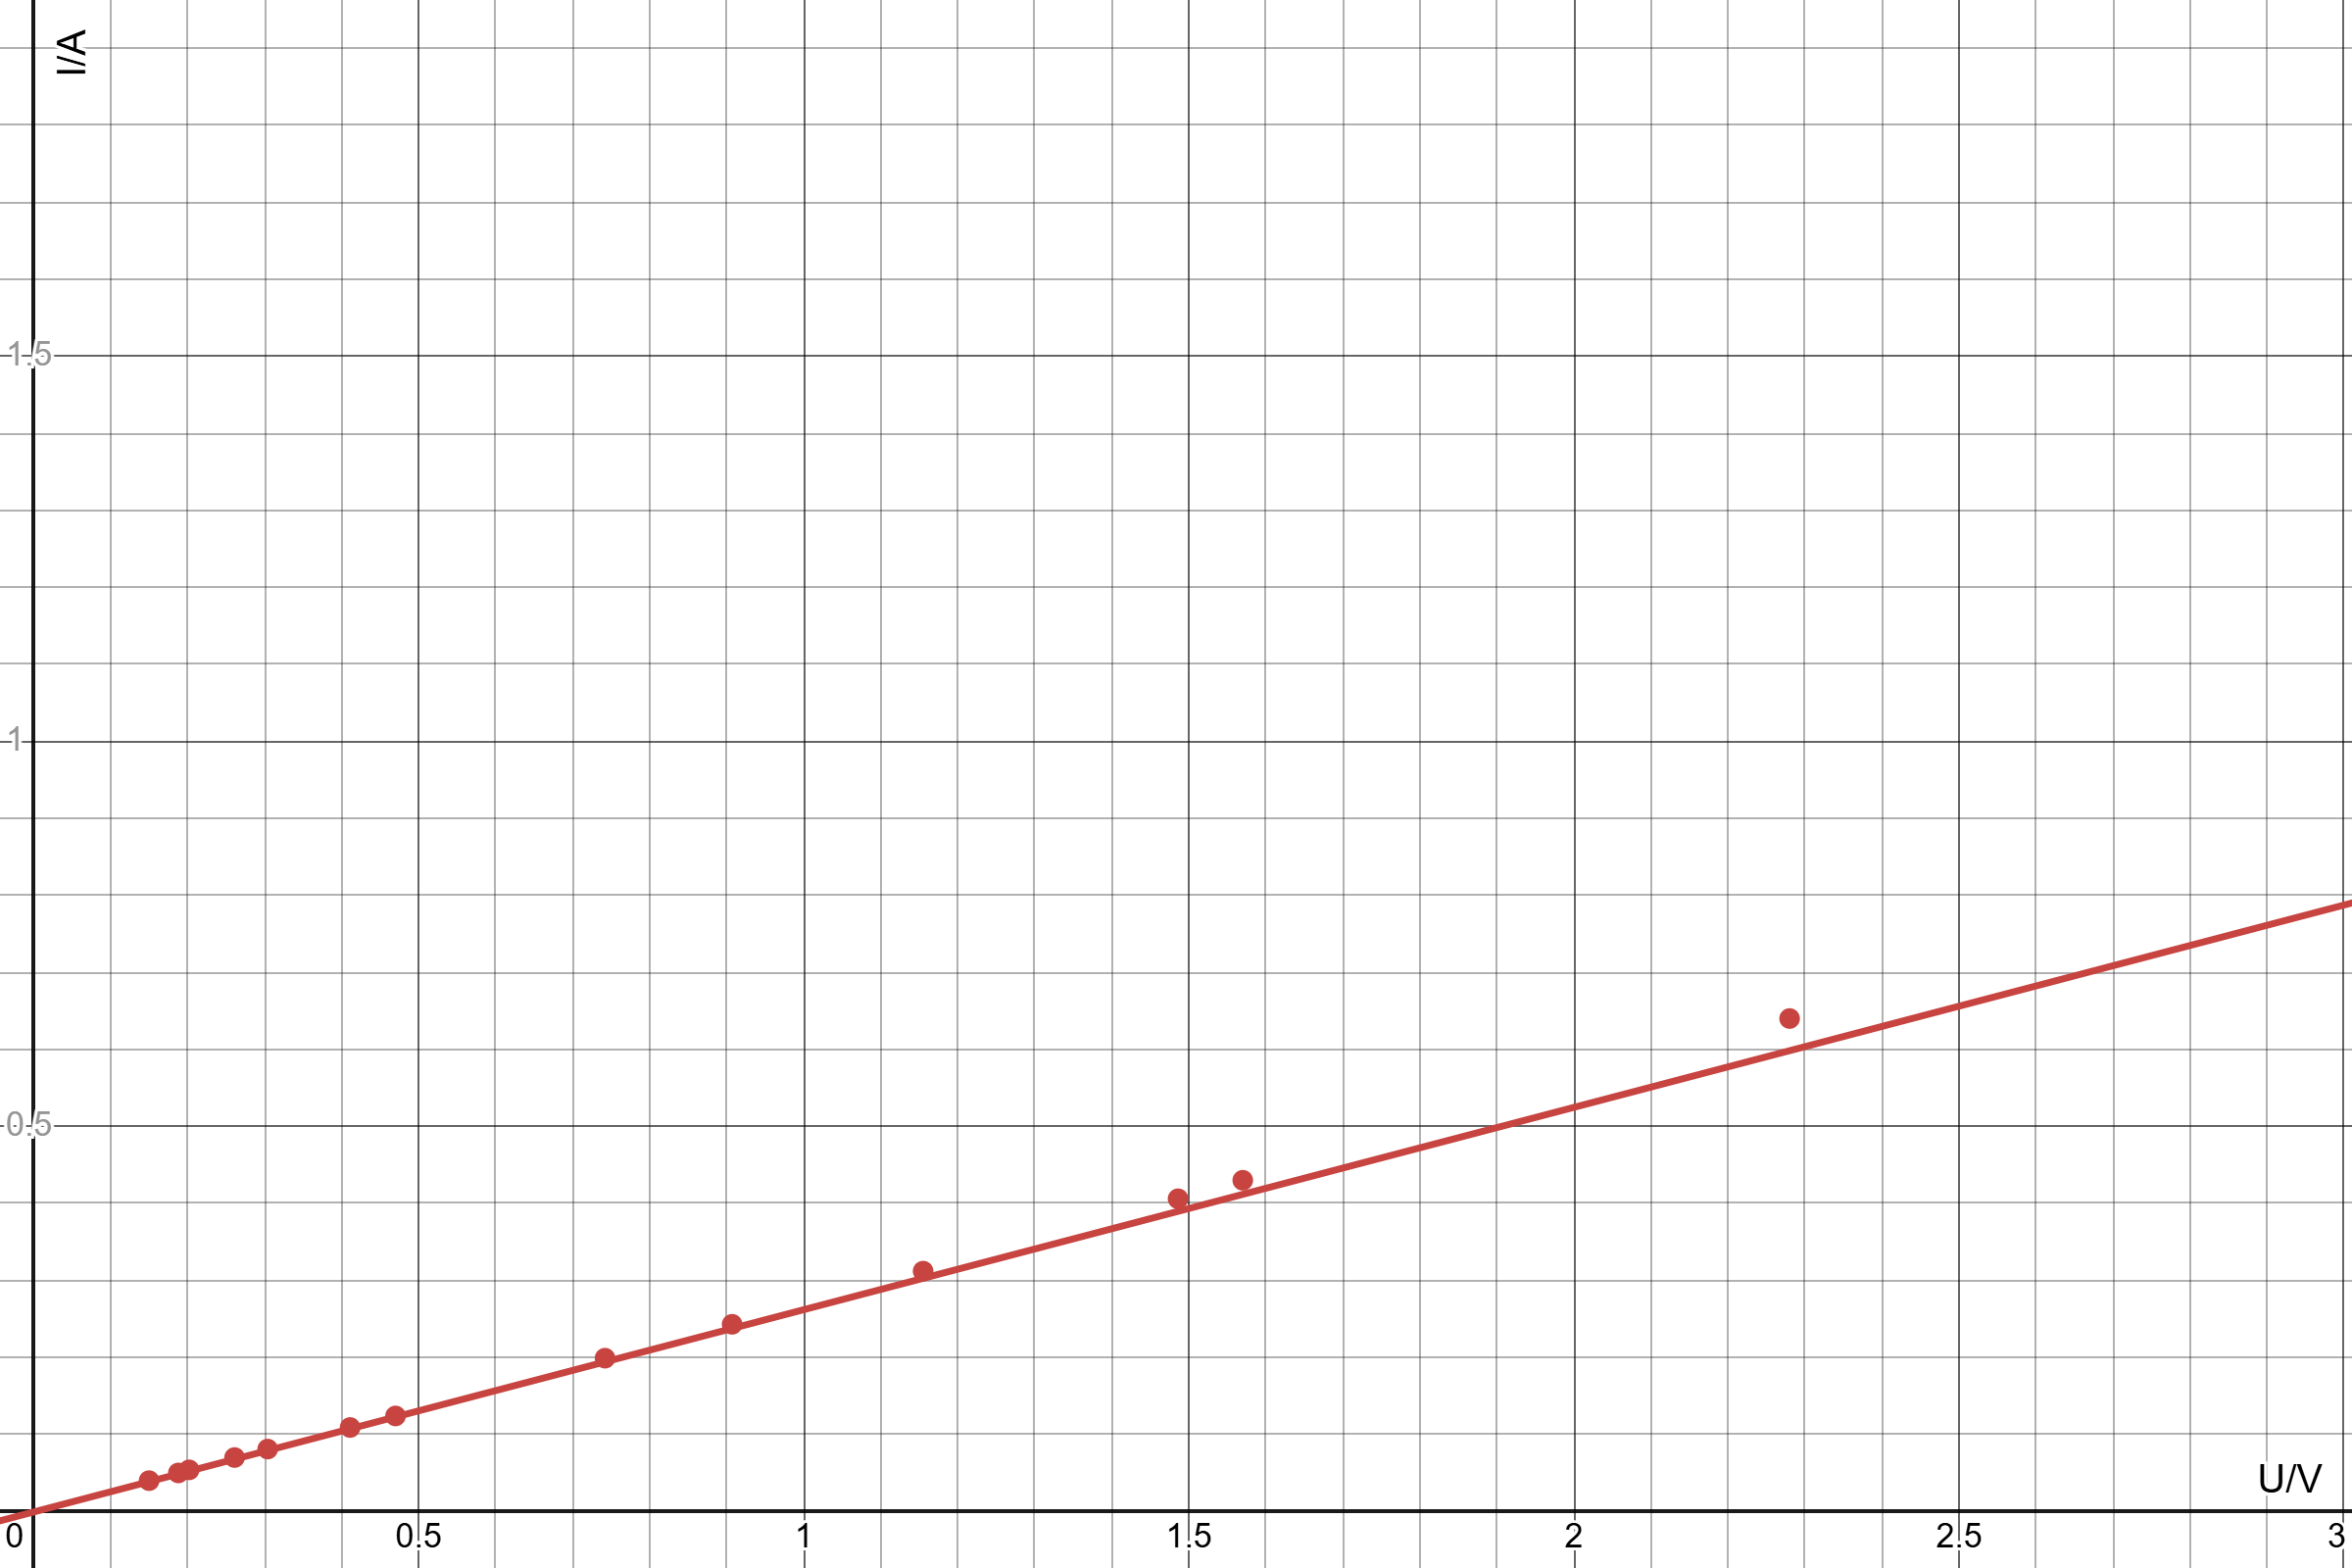
\includegraphics[scale=0.15]{Problem_3/Figs_P3/ExpSol1.PNG}
    \caption{}
    \label{fig:S3_01}
\end{figure}
\item Trong trạng thái cân bằng, ta viết được phương trình cân bằng nhiệt: 
\begin{equation}
\dfrac{U^2}{R_0(1 + \alpha \Delta T)} = \beta \Delta T.
\end{equation}
Giải phương trình bậc hai cho sự chênh lệch nhiệt độ dẫn đến
\begin{align}
\frac{U^2}{R_0} &= \beta \Delta T (1 + \alpha \Delta T) \Rightarrow \alpha \beta (\Delta T)^2 + \beta \Delta T - \frac{U^2}{R_0} = 0. \\
\Delta T &= \frac{-\beta \pm \sqrt{\beta^2 + 4 \frac{U^2}{R_0} \alpha \beta}}{2\alpha \beta}.
\end{align}
Từ dữ liệu thu được suy ra rằng hệ số nhiệt độ của điện trở graphit là âm, do đó nghiệm nhỏ hơn sẽ là nghiệm với dấu + . Do đó, phương trình mô tả đặc tính U-I lý thuyết có dạng:
\begin{equation}
I = \dfrac{U}{R_0(1 + \alpha \Delta T)} = \dfrac{U}{R_0\left(1 + \frac{-\beta + \sqrt{\beta^2 + 4 \frac{U^2}{R_0} \alpha \beta}}{2\beta}\right)} \approx \frac{U}{R_0\left(1 + \frac{U^2}{R_0} \frac{\alpha}{\beta}\right)} \approx \frac{U}{R_0} \left[1 - \frac{U^2}{R_0} \frac{\alpha}{\beta}\right].
\end{equation}
\item Từ số liệu thí nghiệm đã cho, ta tính được điện trở của miếng graphite: $R_0=3.78 \Omega$. Để chính xác nhất có thể, ta se chỉ xử lý những số liệu thu được ở giá trị điện thế thấp (<0.5V) vì ở thời điểm đó, thanh graphite sẽ chưa bị nóng lên quá nhiều.\\
Điện trở suất của miếng graphite: \\
\begin{equation}
\boxed{
    \rho=\dfrac{\pi d^2}{4l}R_0=5.93 \cdot 10^{-5} \left( \Omega\cdot \si{m}\right).
    }
\end{equation}
\item Trong trạng thái cân bằng, công suất tỏa ra khi dòng điện chạy qua bằng với công suất tổn hao nhiệt:
\begin{equation}
P = \beta \Delta T \quad \Rightarrow \quad \Delta T = \frac{P}{\beta}.
\end{equation}
Do đó, sự phụ thuộc của điện trở vào công suất có dạng:
\begin{equation}
\boxed{
R_g = R_0(1 + \alpha \Delta T) = R_0\left(1 + \dfrac{\alpha}{\beta} P\right).
}
\end{equation}
\item Sự phụ thuộc của điện trở vào công suất tiêu tốn được biểu diễn trong hình vẽ.
\begin{figure}[H]
    \centering
    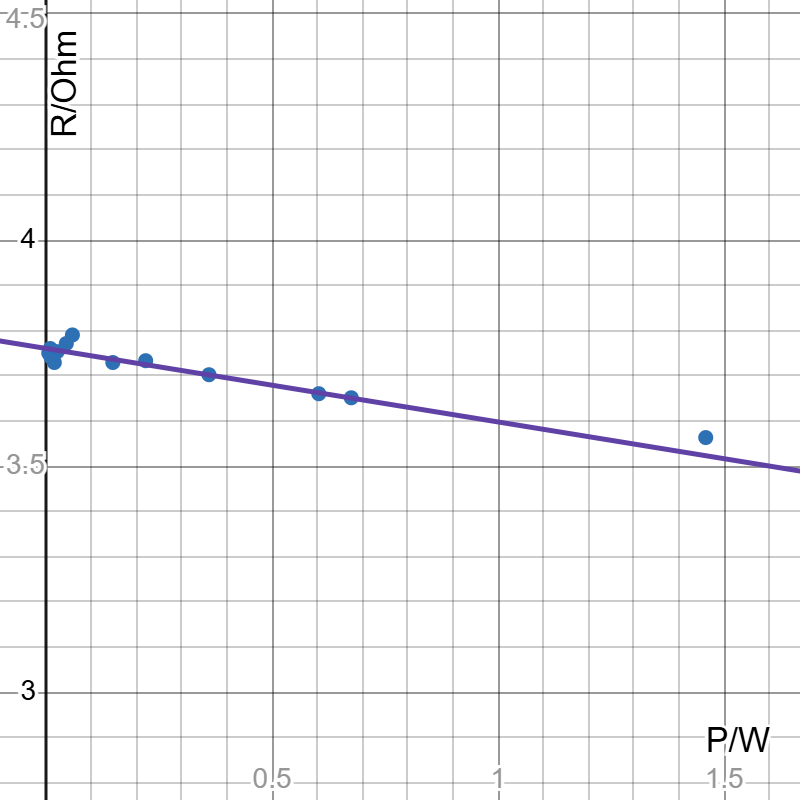
\includegraphics[scale=0.45]{Problem_3/Figs_P3/ExpSol2.PNG}
    \caption{}
    \label{fig:S3_02}
\end{figure}
Tính tuyến tính của sự phụ thuộc này được quan sát thấy ở các công suất lớn hơn $0,2W$. \\
Đặt biểu thức biểu diễn sự phụ thuộc tuyến tính giữa R và P là $R = aP + b$. Từ đồ thị, ta tính xấp xỉ được $a = 0.16 \Omega \cdot W^{-1}$, $b = 3.76 \Omega$, do đó, hệ số $\gamma$ trong công thức ở phần (e) được tính như sau: \\
\begin{equation}
\boxed{
\gamma = \frac{a}{b} = 0.035 \left(\si{W}^{-1}\right).
}
\end{equation}
\newpage 
\item Từ bảng số liệu đã cho, ta vẽ được đồ thị như sau: 
\begin{figure}[H]
    \centering
    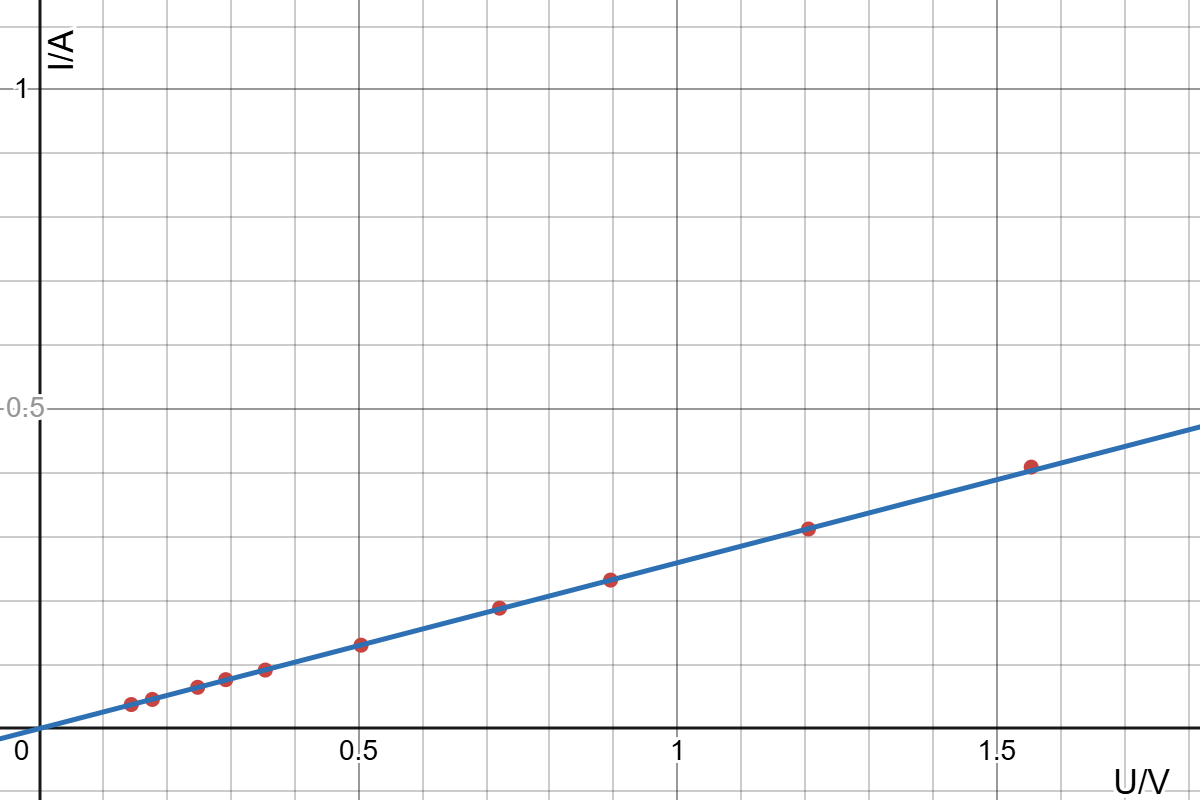
\includegraphics[scale=0.4]{Problem_3/Figs_P3/ExpSol3.PNG}
    \caption{}
    \label{fig:S3_03}
\end{figure}
Trong đồ thị này cũng có một sự phi tuyến tính nhỏ khi công suất tăng. Do đó, để tính điện trở ở nhiệt độ không, chỉ nên sử dụng một vài điểm ban đầu với điện trở thấp. Tính toán cho năm điểm đầu tiên dẫn đến giá trị sau:
\begin{equation}
R_g = 3.88 \left(\Omega\right).
\end{equation}
Vì giá trị này phải tuân theo công thức $R_g = R_0(1 + \alpha \Delta T)$, hệ số nhiệt độ của điện trở có thể được tính như sau:
\begin{equation}
\boxed{
\alpha = \frac{1}{\Delta T} \left(\frac{R_g}{R_0} - 1\right)= -1.3 \cdot 10^{-3} \left(\si{K}^{-1}\right).
}
\end{equation}
\newpage
\textbf{Phổ điểm}
    \begin{center}
    \begin{tabular}{|c|p{8cm}|c|}
    \hline
    \multicolumn{1}{|l|}{Phần} & Nội dung & Điểm thành phần \\ 
    \hline
\multirow{1}{*}{(a)} & Giải thích đúng cách đo.                                                                                  & 0.25             
                                \\ \hline
\multirow{1}{*}{(b)} & Vẽ đúng đồ thị.                                                                                & 0.25             
                                \\ \hline
\multirow{4}{*}{(c)} & Viết đúng phương trình cân bằng nhiệt.                               
                     & 0.25            \\ \cline{2-3}
                     & Giải đúng phương trình bậc 2 cho sự chênh lệch nhiệt độ.         
                     & 0.25            \\ \cline{2-3}
                     & Chọn đúng nghiệm nhỏ hơn                
                     & 0.25            \\ \cline{2-3}
                     & Viết đúng biểu thức cuối của I theo các đại lượng              
                     & 0.25           
                     \\ \hline
\multirow{2}{*}{(d)} & Xử lý được số liệu và thu được điện trở miếng graphite (cho phép sai số $0.03\Omega$)                            
                     & 0.5            \\ \cline{2-3}
                     & Tính được đúng điện trở suất từ điện trở đã được tính được    
                     & 0.25             
                     \\ \hline
\multirow{1}{*}{(e)} & Viết đúng biểu thức $R_g$                                                                            & 0.25          
\\ \hline     
\multirow{2}{*}{(f)} & Vẽ được đồ thị chuẩn                                                                        & 0.25    \\ \cline{2-3}     
& Từ đồ thị xấp xỉ được hai giá trị a và b và tính được $\gamma$                                                   & 0.5  
                                \\ \hline
\multirow{1}{*}{(g)} & Vẽ được đồ thị chuẩn                                                                        & 0.25     \\ \cline{2-3}     
& Từ đồ thị tính được $R_g$                                                   
& 0.25     \\ \cline{2-3}
& Tính được đúng giá trị của $\alpha$                                                   
& 0.25     \\ \hline                                


    \end{tabular}
    \end{center}
\end{enumerate}

\begin{flushright}
   (biên soạn bởi Meng)
\end{flushright}
\newpage

%%%%%%%%%% CÂU 4 %%%%%%%%%%
{\normalcolor{\textbf{CÂU IV. (4.0 điểm)}}}
\setcounter{equation}{0}


Một mặt bàn hình vuông có khối lượng m (trọng lượng phân bố đều) và cạnh dài a được treo bằng 4 sợi dây xích đồng nhất và có chiều dài L. Đặt hệ tọa độ có gốc đặt tại trung tâm của bàn, các sợi dây được gắn cố định vào mặt bàn tại 4 góc và các điểm có tọa độ $\left(\pm \frac{a}{2},\pm\frac{a}{2}\right)$. 
\begin{figure}[H]
    \centering
    \tikzset{every picture/.style={line width=0.75pt}} %set default line width to 0.75pt        

\begin{tikzpicture}[x=0.75pt,y=0.75pt,yscale=-1,xscale=1]
%uncomment if require: \path (0,429); %set diagram left start at 0, and has height of 429

%Shape: Rectangle [id:dp43479829147458826] 
\draw   (150,200) -- (350,200) -- (350,220) -- (150,220) -- cycle ;
%Shape: Rectangle [id:dp26418096458424434] 
\draw   (350,200) -- (442.03,122.78) -- (442.03,143.14) -- (350,220) -- cycle ;
%Straight Lines [id:da6303516163988201] 
\draw    (240.42,122.25) -- (442.46,122.25) ;
%Straight Lines [id:da2435007903542885] 
\draw    (149.96,200) -- (240.78,122.42) ;
%Straight Lines [id:da12397037243108167] 
\draw    (112.03,23.59) -- (461.43,23.59) ;
%Shape: Axis 2D [id:dp11255839884999319] 
%\draw [dashed] (121.01,156.7) -- (506.99,156.7)(409.6,45.33) -- (177.57,277.36) (504.99,151.7) -- (506.99,156.7) -- (494.99,161.7) (397.6,52.33) -- (409.6,45.33) -- (407.6,52.33)  ;
%Straight Lines [id:da6910540327628811] 
\draw    (150,200) -- (150,23.64) ;
%Straight Lines [id:da778712219228807] 
\draw    (241,122.34) -- (241,23.55) ;
%Straight Lines [id:da014093703911455924] 
\draw    (442,122.34) -- (442,22.35) ;
%Straight Lines [id:da13741894893199325] 
\draw    (350,200) -- (350,104.51) -- (350,23.64) ;


% Text Node

\filldraw(255.21,171.12) circle(2.5)node [anchor=north east][align=right] {M};

\draw [<->](150,240) -- (250,240)node[below]{a} -- (350,240) ;

\draw [dashed] [->] (165.23,161.12) -- (435.23,161.12);
\draw [dashed] [->] (222.42,232.62) -- (367.93,87.11);
\filldraw(295.21,161.12) circle(2.5) node [anchor=north west][align=left] {O};
\end{tikzpicture}
    \caption{}
    \label{fig:P4_01}
\end{figure}
Giả sử trọng lượng của các dây xích là không đáng kể so với trọng lượng của mặt bàn.
Bên trên mặt bàn, ta đặt một chậu cây có khối lượng M. Đối với bài này, ta coi đế của chậu cây là rất nhỏ so với mặt bàn và coi chậu là một chất điểm M.
\begin{enumerate} [label=(\alph*)]
    \item Khi chậu cây đặt đúng tại tâm bàn và đang cân bằng, giả sử dây không giãn, hãy chứng minh lực căng trong mỗi dây được tính theo công thức:
    \begin{equation}
        T = \dfrac{(m+M)g}{4}
    \end{equation}
\item 
\begin{enumerate}[label=(\roman*)]
\item Đặt chậu cây tại vị trí (x,y), hãy tìm lực căng của từng dây. Coi rằng các dây đều
tuân theo định luật Hooke: $T = k \cdot\Delta{x}$ với $\Delta{x}$ là độ dãn của dây. Cho rằng hệ số đàn hồi k của dây là rất lớn, giới hạn đàn hồi của dây là đủ nhỏ để độ nghiêng của mặt bàn là không đáng kể.
\item Khi không chịu bắt cứ lực căng nào, dây sẽ bị chùng, tìm những vị trí  đặt chậu cây M trên bàn thoả mãn.
\item Dây sẽ bị đứt khi $\Delta{x}>\Delta{l_0}$, tìm quỹ tích các vị trí đặt chậu cây để hệ cân bằng.
\end{enumerate}
\end{enumerate}
\newpage
\begin{center}
\normalcolor{\textbf{Bài giải}}
\end{center}

    \begin{enumerate}[label=(\alph*)]
    \item
    Khi chậu M đặt tại gốc tọa độ O $\left(0, 0\right)$ là trọng tâm của bàn, vì các dây treo là giống nhau nên trọng lực kéo căng các dây là bằng nhau.
    \\
    Lực căng các dây là:
    \begin{equation}
        T_1= T_2= T_3=T_4=T.
    \end{equation}
    Điệu kiện cân bằng là tổng các lực căng phải có độ lớn bằng trọng lực hệ vật:
    \begin{equation}
        |\vec{T_1}| + |\vec{T_2}| + |\vec{T_3}| +|\vec{T_4}| = |\vec{P}|.
    \end{equation}
    \begin{equation}    
        \Longrightarrow 4T = (m+M)\cdot g.
    \end{equation}
    \begin{equation}   
        \boxed{
        \Longrightarrow T = \dfrac{(m+M)\cdot g}{4}.
        }
    \end{equation}
    \item 
    \begin{enumerate}[label=(\roman*)]
    \item
        \begin{figure}[H]
    \centering
    \tikzset{every picture/.style={line width=0.75pt}} %set default line width to 0.75pt        

\begin{tikzpicture}[x=0.75pt,y=0.75pt,yscale=-1,xscale=1]
%uncomment if require: \path (0,429); %set diagram left start at 0, and has height of 429

%Shape: Rectangle [id:dp43479829147458826] 
\draw   (147.34,176.52) -- (344.82,208.15) -- (341.55,228.58) -- (144.07,196.95) -- cycle ;
%Shape: Rectangle [id:dp26418096458424434] 
\draw   (344.94,208.08) -- (447.9,146.46) -- (444.68,166.56) -- (341.71,228.19) -- cycle ;
%Straight Lines [id:da6303516163988201] 
\draw    (248.92,114.05) -- (448.42,146) ;
%Straight Lines [id:da2435007903542885] 
\draw    (147.3,176.51) -- (249.25,114.27) ;
%Shape: Rectangle [id:dp43479829147458826] 
%\draw   (150,200) -- (350,200) -- (350,220) -- (150,220) -- cycle ;
%Shape: Rectangle [id:dp26418096458424434] 
%\draw   (350,200) -- (442.03,122.78) -- (442.03,143.14) -- (350,220) -- cycle ;
%Straight Lines [id:da6303516163988201] 
%\draw    (240.42,122.25) -- (442.46,122.25) ;
%Straight Lines [id:da2435007903542885] 
%\draw    (149.96,200) -- (240.78,122.42) ;
%WALL 
\draw    (112.03,23.59) -- (461.43,23.59) ;
%Shape: Axis 2D [id:dp11255839884999319] 
%\draw [dashed] (121.01,156.7) -- (506.99,156.7)(409.6,45.33) -- (177.57,277.36) (504.99,151.7) -- (506.99,156.7) -- (494.99,161.7) (397.6,52.33) -- (409.6,45.33) -- (407.6,52.33)  ;
%Straight Lines [id:da6910540327628811] 
\draw  [->]  (147.34,176.52) -- (147.34,53.64) node [right] {$\vec{T_4}$} ;
\draw    (147.34,176.52) -- (147.34,23.64) ;
%Straight Lines [id:da778712219228807] 
\draw  [->]  (248.92,114.27) -- (248.92,53.64) node [left] {$\vec{T_1}$} ;
\draw    (248.92,114.27) -- (248.92,23.55) ;
%Straight Lines [id:da014093703911455924]
\draw  [->]  (447.9,146.46) -- (447.9,53.64) node [right] {$\vec{T_2}$} ;
\draw    (447.9,146.46) -- (447.9,22.35) ;
%Straight Lines [id:da13741894893199325] 
\draw    (344.82,200) -- (344.82,104.51) -- (344.82,23.64) ;
\draw  [->]  (344.82,208.15) -- (344.82,53.64) node [right] {$\vec{T_3}$} ;


% Text Node

\filldraw(255.21,136.12) circle(2.5)node [anchor=north east][align=right] {$M(x;y)$};
\draw[dashed][->](255.21,136.12) -- (255.21,251.12) node [right]{$\vec{P_1}$};

\draw[thick]  [->] (125.23,161.12) -- (475.23,161.12) node [right]{x};
\draw[ thick]  [->] (222.42,232.62) -- (367.93,87.11) node [right] {y};
\draw[ thick] [dashed](295.21,161) -- (295.21,271);
\draw [dashed][->](295.21,201) -- (295.21,251) node [right] {$\vec{P_2}$};
\draw[ thick]  [->] (295.21,161) -- (295.21,51) node [above] {z};
\filldraw(295.21,161) circle(2.5) node [anchor=north west][align=left] {O};
\end{tikzpicture}
    \caption{}
    \label{fig:S4_01}
    \end{figure}
    Chậu M được coi là chất điểm đặt tại $M \left( x;y \right)$ với hệ trục tọa độ gắn với khối tâm của bàn nằm ngang.
    Các điều kiện cân bằng của hệ vật:
    \begin{enumerate} [label=(\arabic*)]
    \item Cân bằng lực theo phương thẳng đứng: Tổng độ lớn các lực căng dây phải bằng trọng lượng của hệ vật:
    \begin{equation}
        \vec{T_1} + \vec{T_2} + \vec{T_3} +\vec{T_4} = \vec{P}.
    \end{equation}
    Tức:
    \begin{equation}
        |\vec{T_1}| + |\vec{T_2}| + |\vec{T_3}| +|\vec{T_4}| = |\vec{P}|.
    \end{equation}
    hay:
    \begin{equation}
        T_1+T_2+T_3+T_4 = (m+M) \cdot g.
    \end{equation}
        \item
    Tính đàn hồi của dây:
    Vì hệ số đàn hồi của dây K là rất lớn và giới hạn đàn hồi không đáng kể, bàn chuyển dịch một đoạn rất nhỏ theo phương thẳng đứng.
    \\
    Xét sự chuyển vị theo phương thẳng đứng (Oz) tại mỗi đỉnh của bàn:
            \begin{figure}[H]
    \centering
    \tikzset{every picture/.style={line width=0.75pt}} %set default line width to 0.75pt        
\begin{tikzpicture}
       \node (a) at (0,0)
         {
\begin{tikzpicture}[x=0.75pt,y=0.75pt,yscale=-1,xscale=1]
\draw [->] (165.23,161.12) -- (435.23,161.12) node [right]{y};
\draw(295.21,161) -- (295.21,271);
\draw [->] (295.21,161) -- (295.21,51) node [above] {z};
%\draw (295.21,161) circle (7.5);
%\draw (295.21,161)node[anchor=south east] {x};
\filldraw(295.21,161) circle(2.5) node [anchor=north west][align=left] {O};
\draw   (200,175) -- (400,200) -- (400,205) -- (200,180) -- cycle ;
\draw[dashed](400,205.5) -- (295.21,205.5) node[left]{$z_y$};
\draw (295.21,180) node[left] {$z_0$};
\draw
(210,176) to [in=5](210,161.12);
\draw
(215,176.5) to [in=5](215,161.12)
;
\draw (220,171.12) node [right] {$\theta y$};
\draw [dashed] [<->](400,205) -- (400,161.12);
\draw (400, 180) node[right]{$\Delta z_x$};
\end{tikzpicture}
};
\node (b) at (a.east) [xshift=150]
{
%\end{tikzpicture}
%    \caption{}
%    \label{fig:S4_02}
%    \end{figure}
%            \begin{figure}[H]
%    \centering
    \tikzset{every picture/.style={line width=0.75pt}} %set default line width to 0.75pt        

\begin{tikzpicture}[x=0.75pt,y=0.75pt,yscale=-1,xscale=1]
\draw [->] (165.23,161.12) -- (435.23,161.12) node [right]{x};
\draw(295.21,161) -- (295.21,271);
\draw [->] (295.21,161) -- (295.21,51) node [above] {z};
%\draw (295.21,161) circle (7.5) 
%\draw (295.21,161) node[anchor=south east] {y};
\filldraw(295.21,161) circle(2.5) node [anchor=north west][align=left] {O};
\draw   (200,175) -- (400,200) -- (400,205) -- (200,180) -- cycle ;
\draw
(210,176) to [in=5](210,161.12);
\draw
(215,176.5) to [in=5](215,161.12)
;
\draw (220,171.12) node [right] {$\theta x$};
\draw[dashed](400,205.5) -- (295.21,205.5);
\draw (295.21,205.5) node[left]{$z_x$};
\draw [dashed] [<->](400,205) -- (400,161.12);
\draw (400, 180) node[right]{$\Delta z_y$};
\draw (295.21,180) node[left] {$z_0$};
\end{tikzpicture}
 };
 \end{tikzpicture}
    \caption{}
    \label{fig:S4_02}
    \end{figure}
    Vì góc nghiêng của bàn rất nhỏ và có thể xem như không nghiêng, ta có thể xem sự chuyển vị là tuyến tính:
    \\Tại vị trí $\left(-\dfrac{a}{2};\dfrac{a}{2}\right)$:
    \begin{equation}
        \Delta z_1 = z_0 +\dfrac{a}{2} \theta y -\dfrac{a}{2} \theta x.
    \end{equation}
    Tại vị trí $\left(\dfrac{a}{2};\dfrac{a}{2}\right)$:
    \begin{equation}
        \Delta z_2 = z_0 +\dfrac{a}{2} \theta y +\dfrac{a}{2} \theta x.
    \end{equation}
    Tại vị trí $\left(\dfrac{a}{2};-\dfrac{a}{2}\right)$:
    \begin{equation}
        \Delta z_3 = z_0 -\dfrac{a}{2} \theta y 
 +\dfrac{a}{2} \theta x.
    \end{equation}
    Tại vị trí $\left(-\dfrac{a}{2};-\dfrac{a}{2}\right)$:
    \begin{equation}
        \Delta z_4 = z_0 -\dfrac{a}{2} \theta y -\dfrac{a}{2} \theta x.
    \end{equation}
    Áp dụng định luật Hooke cho các dây treo dãn đã cho, lực căng dây i có độ lớn:
    \begin{equation}
        T_i = k \cdot \Delta z_i \left( i \in N^* |1 \le i \le 4 \right).
    \end{equation}
    với độ dãn của dây là $\Delta z_i$.
    \item Do độ nghiêng của bàn là nhỏ, ta bỏ qua momen gây bởi lực ma sát nghỉ sinh ra để giữ cân bằng cho vật, có độ lớn tỉ lệ với góc nghiêng. \newline Momen lực gây ra bởi các lực căng dây có thể được phân tích thành hai thành phần.
    \newline
    Cân bằng moment lực đối với M trên trục Ox:
    \begin{equation}
        \dfrac{a}{2}\vec{T_1}+\dfrac{a}{2}\vec{T_2}+\dfrac{a}{2}\vec{T_3}+\dfrac{a}{2}\vec{T_4} =  |y|\cdot \vec{P_1}.
    \end{equation}
    Trên trục Ox:
    \begin{equation}
    \Longrightarrow    
    -\dfrac{a}{2}T_1+\dfrac{a}{2}T_2+\dfrac{a}{2}T_3-\dfrac{a}{2}T_4 = Mgy.
    \end{equation}
    \begin{equation}
    \Longleftrightarrow   
    T_2 +T_3 - T_1-T_4 = \dfrac{2Mgy}{a}.
    \end{equation}
    \item
    Cân bằng moment đối với vật M trên trục Oy:
    \begin{equation}
        \dfrac{a}{2}\vec{T_1}+\dfrac{a}{2}\vec{T_2}+\dfrac{a}{2}\vec{T_3}+\dfrac{a}{2}\vec{T_4} =  |x|\cdot \vec{P_1}.
    \end{equation}
    Trên trục Oy:
    \begin{equation}
    \Longrightarrow    
    -\dfrac{a}{2}T_1-\dfrac{a}{2}T_2+\dfrac{a}{2}T_3+\dfrac{a}{2}T_4 = Mgx.
    \end{equation}
    \begin{equation}
    \Longleftrightarrow   
    T_3 +T_4- T_1-T_2 = \dfrac{2Mgx}{a}.
    \end{equation}
    \end{enumerate}
    Kết hợp điều kiện (1.):
    \begin{equation}
        T_1 + T_2 +T_3 +T_4 = k \cdot (z_1 +z_2+z_3+z_4) = k \cdot 4z_0 = (m+M)\cdot g.
    \end{equation}
    Do vậy:
    \begin{equation}
        z_0 = \dfrac{(m+M)\cdot g}{4k}.
    \end{equation}
    Kết hợp điều kiện (2.):
    \begin{equation}
        T_2 +T_3 - T_1 -T_4 = k \cdot (z_2 +z_3 - z_1 - z_4)
    \end{equation}
    \begin{equation} 
        = k \cdot \left[(a \cdot \theta y + a \cdot \theta x) + (-a \cdot \theta y + a \cdot \theta x) - (a \cdot \theta y - a \cdot \theta x) - (-a \cdot \theta y - a \cdot \theta x)\right]
    \end{equation}
    \begin{equation}
        = k \cdot 2a \theta y = \dfrac{2Mgy}{a}.
    \end{equation}
    Vì thế:
    \begin{equation}
        \theta y = + \dfrac{Mgy}{ka^2}.
    \end{equation}
    Kết hợp điều kiện (3.):
    \begin{equation}
        T_3 +T_4 - T_1 -T_2 = k \cdot (z_3 +z_4 - z_1 - z_2)
    \end{equation}
    \begin{equation} 
        = k \cdot \left[(-a \cdot \theta y + a \cdot \theta x) + (-a \cdot \theta y - a \cdot \theta x) - (a \cdot \theta y - a \cdot \theta x) - (a \cdot \theta y + a \cdot \theta x)\right]
    \end{equation}
    \begin{equation}
        = k \cdot 2x \theta y = \dfrac{2Mgx}{a}.
    \end{equation}
    Vì thế:
    \begin{equation}
        \theta x = + \dfrac{Mgx}{ka^2}.
    \end{equation}
    Từ $z_0 = \dfrac{(m +M)\cdot g}{4k}$; $\theta y = \dfrac {Mgy}{ka^2}$; $\theta x = \dfrac {Mgx}{ka^2}$ thế vào biểu thức lực căng từ dây $T_i=k \cdot \Delta z_i$, ta được:
    
    \begin{equation}
    \boxed{
        T_1 = k \cdot \left[ \dfrac{(m+M)g}{4k}+\dfrac{a}{2} \cdot \dfrac{Mgy}{ka^2}-\dfrac{a}{2}\cdot \dfrac{Mgx}{ka^2}\right] = \dfrac{(m+M)g}{4}+\dfrac{Mgy}{2a}-\dfrac{Mgx}{2a}.
            }
    \end{equation}
    \begin{equation}
    \boxed{
        T_2 = k \cdot \left[ \dfrac{(m+M)g}{4k}+\dfrac{a}{2} \cdot \dfrac{Mgy}{ka^2}+\dfrac{a}{2}\cdot \dfrac{Mgx}{ka^2}\right] = \dfrac{(m+M)g}{4}+\dfrac{Mgy}{2a}+\dfrac{Mgx}{2a}.
            }
    \end{equation}
    \begin{equation}
    \boxed{
        T_3 = k \cdot \left[ \dfrac{(m+M)g}{4k}-\dfrac{a}{2} \cdot \dfrac{Mgy}{ka^2}+\dfrac{a}{2}\cdot \dfrac{Mgx}{ka^2}\right] = \dfrac{(m+M)g}{4}-\dfrac{Mgy}{2a}+\dfrac{Mgx}{2a}.
            }
    \end{equation}
    \begin{equation}
    \boxed{
        T_4 = k \cdot \left[ \dfrac{(m+M)g}{4k}-\dfrac{a}{2} \cdot \dfrac{Mgy}{ka^2}-\dfrac{a}{2}\cdot \dfrac{Mgx}{ka^2}\right] = \dfrac{(m+M)g}{4}-\dfrac{Mgy}{2a}-\dfrac{Mgx}{2a}.
            }
    \end{equation}
\item Dây sẽ bị chùng khi không có lực nào căng hai đầu dây. Vì bàn có khối lượng $m>0$ nên không có trường hợp hai dây trùng một lúc.
\\$\longrightarrow$ Chỉ một dây có thể trùng một lúc, tức $T_i \le 0$
Với $i =1$ (Dây 1 bị trùng), $T_1 \le 0$:
\begin{equation}
\Longrightarrow\dfrac{(m+M)g}{4}+\dfrac{Mgy}{2a}-\dfrac{Mgx}{2a} \le 0.
\end{equation}
\begin{equation}
\label{eq:S4_01}
\Longrightarrow
y \le x -\dfrac{(m+M)a}{2M}.
\end{equation}
Với $i =2$, $T_2 \le 0$:
\begin{equation}
\Longrightarrow\dfrac{(m+M)g}{4}+\dfrac{Mgy}{2a}+\dfrac{Mgx}{2a} \le 0.
\end{equation}
\begin{equation}
\label{eq:S4_02}
\Longrightarrow
y \le -x -\dfrac{(m+M)a}{2M}.
\end{equation}
Với $i =3$, $T_3 \le 0$:
\begin{equation}
\Longrightarrow\dfrac{(m+M)g}{4}-\dfrac{Mgy}{2a}+\dfrac{Mgx}{2a} \le 0.
\end{equation}
\begin{equation}
\label{eq:S4_03}
\Longrightarrow
y \ge x + \dfrac{(m+M)a}{2M}.
\end{equation}
Với $i =4$, $T_4 \le 0$:
\begin{equation}
\Longrightarrow\dfrac{(m+M)g}{4}-\dfrac{Mgy}{2a}-\dfrac{Mgx}{2a} \le 0.
\end{equation}
\begin{equation}
\label{eq:S4_04}
\Longrightarrow
y \ge -x + \dfrac{(m+M)a}{2M}.
\end{equation}
Tập hợp điểm M đặt chậu trên bàn là hình vuông tạo bởi các đỉnh:
\\$\left(-\dfrac{a}{2},\dfrac{a}{2}\right)$;$\left(\dfrac{a}{2},\dfrac{a}{2}\right)$;$\left(\dfrac{a}{2};\dfrac{a}{2}\right)$;$\left(-\dfrac{a}{2},\dfrac{a}{2}\right)$.
Xét $i=4$ (dây 4 bị trùng là trường hợp điển hình)
\begin{equation}
   \begin{cases}
   y = -x + \dfrac{(m+M)a}{2M}
   \\
   y=\dfrac{a}{2}
   \end{cases}
\end{equation}
\begin{equation}
    \Longrightarrow x=\dfrac{a}{2}\cdot \dfrac{m}{M}.
\end{equation}
\begin{equation}
   \begin{cases}
   y = -x + \dfrac{(m+M)a}{2M}
   \\
   x=\dfrac{a}{2}
   \end{cases}
\end{equation}
\begin{equation}
    \Longrightarrow y=\dfrac{a}{2}\cdot \dfrac{m}{M}.
\end{equation}
$\Longrightarrow$ $\begin{cases}
\text{M nằm ngoài bàn: $m>M;m,M>0$}
\\
\text{M thỏa mãn: $m \le M ;m,M >0$}
\end{cases}$
\\
Ta thấy rằng:
\\Với $m>M$ (bàn có khối lượng lớn hơn chậu cây) thì không có vị trí đặt trên bàn chậu M để dây bị chùng.
\\ Với $m=M$, các điểm thỏa mãn là các đỉnh treo dây của bàn.
\\Nếu bàn có khối lượng $m<M$, quỹ tích điểm $M(x;y)$ thỏa mãn đề bài là vùng giao nhau trong không gian bàn với các bất phương trình \eqref{eq:S4_01}, \eqref{eq:S4_02}, \eqref{eq:S4_03}, \eqref{eq:S4_04}.

\begin{figure}[H]
    \centering
    \tikzset{every picture/.style={line width=0.75pt}} %set default line width to 0.75pt       
\begin{tikzpicture}[x=0.75pt,y=0.75pt,yscale=-1,xscale=1]
\draw [->] (115.23,161.12) -- (485.23,161.12) node [right]{x};
\draw(295.21,161) -- (295.21,321);
\draw [->] (295.21,161) -- (295.21,1) node [above] {y};
\draw (295.21,161) circle (7.5) node[anchor=south west] {z};
\filldraw(295.21,161) circle(2.5) node [anchor=south east] {O};
\draw (395.21,61) -- (395.21,261)--(195.21,261)--(195.21,61)--(395.21,61);
\draw[dashed] (420.21,161)--(295.21,36)--(170.21,161)--(295.21,286)--(420.21,161);
\filldraw [fill=gray!20] (195.21,185.12) -- (195.21,261) -- (271,261);
\filldraw [fill=gray!20] (395.21,185.12) -- (395.21,261) -- (319,261);
\filldraw [fill=gray!20] (195.21,137) -- (195.21,61) -- (271,61);
\filldraw [fill=gray!20] (395.21,137) -- (395.21,61) -- (319,61);
\filldraw(295.21,36) circle(2.5) node [anchor=south east] {$y_i$};
\filldraw(420.21,161) circle(2.5) node [anchor=north west] {$x_i$};
\filldraw(195.21,161) circle(1.25) node [anchor=south west] {$-\dfrac{a}2$};
\filldraw(395.21,161) circle(1.25);
\draw (385.21,161) node [anchor=north east]{$\dfrac{a}2$};
\filldraw(295.21,261) circle(1.25) node [anchor=south west] {$-\dfrac{a}2$};
\filldraw(295.21,61) circle(1.25) node [anchor=north east] {$\dfrac{a}2$};
\filldraw(295.21,286) circle(1.25);
\draw (295.21,300) node [anchor=south west] {$-a$};
\filldraw (319,61) circle(1.25) node [anchor=south west] {$\left( \dfrac{a}2 \dfrac{m}{M};\dfrac{a}2 \right)$};
\filldraw (395.21,137) circle(1.25);
\draw (395.21,130)node [right] {$\left( \dfrac{a}2 \dfrac{m}{M};\dfrac{a}2 \right)$};
\end{tikzpicture}
    \caption{
    $\begin{cases}
    \dfrac{a}2 \le |x_i| \le a
    \\
    \\
    \dfrac{a}2 \le |y_i| \le a
    \end{cases}
    $
    ($x_i,y_1$ là giao điểm bất phương trình dây i với trục Ox, Oy)
    }
    \label{fig:S4_03}
    \end{figure}
Nhận xét: Lực căng dây có độ lớn cỡ trọng lượng của bàn. Lực ma sát tỉ lệ với độ nghiêng với khối lượng của chậu. Vậy nếu khối lượng chậu rất nhỏ so với bàn, lực ma sát do đó sẽ vô cùng bé và mô hình ta hoạt động tốt.
    \item
    Dây sẽ bị đứt khi lực căng hai đầu dây vượt qua lực căng tối đa dây có thể chịu $T_{\text{i max}} = \Delta l_0 \cdot k$. Khi đó $M(x;y)$ đặt chậu cân bằng khi $T_i \le \Delta l_0 \cdot k$.
    \\
    Với $i=1$:
    \begin{equation}
        T_1 \le \Delta l_0 \cdot k
    \end{equation}
    \begin{equation}
        \Longrightarrow \dfrac{(m+M)g}4 + \dfrac{Mg}{2a} (y-x)\le k \cdot \Delta l_0.
    \end{equation}
    \begin{equation}
    \label{eq:S4_05}
        \Longrightarrow y - x \le \dfrac{2ak\Delta l_0}{Mg}-\dfrac{(m+M)a}{2M} = \dfrac {a \left[4k \Delta l_0 - (m+M)g\right]}{2Mg}.
    \end{equation}

    Với $i=2$:
    \begin{equation}
        T_2 \le \Delta l_0 \cdot k
    \end{equation}
    \begin{equation}
        \Longrightarrow \dfrac{(m+M)g}4 + \dfrac{Mg}{2a} (y+x)\le k \cdot \Delta l_0.
    \end{equation}
    \begin{equation}
    \label{eq:S4_06}
        \Longrightarrow y - x \le  \dfrac {a \left[4k \Delta l_0 - (m+M)g\right]}{2Mg}.
    \end{equation}

    Với $i=3$:
    \begin{equation}
        T_3 \le \Delta l_0 \cdot k
    \end{equation}
    \begin{equation}
        \Longrightarrow \dfrac{(m+M)g}4 + \dfrac{Mg}{2a} (x-y)\le k \cdot \Delta l_0.
    \end{equation}
    \begin{equation}
    \label{eq:S4_07}
        \Longrightarrow x - y \le  \dfrac {a \left[4k \Delta l_0 - (m+M)g\right]}{2Mg}.
    \end{equation}

    Với $i=4$:
    \begin{equation}
        T_4 \le \Delta l_0 \cdot k
    \end{equation}
    \begin{equation}
        \Longrightarrow \dfrac{(m+M)g}4 + \dfrac{Mg}{2a} (-x-y)\le k \cdot \Delta l_0.
    \end{equation}
    \begin{equation}
    \label{eq:S4_08}
        \Longrightarrow -x - y \le  \dfrac {a \left[4k \Delta l_0 - (m+M)g\right]}{2Mg}.
    \end{equation}
Kết hợp với tập hợp $M(x;y)$ trên bàn:
\\ Xét $i=2$ (Trường hợp dây 2 đứt làm điển hình):
\begin{equation}
    \begin{cases}
       y - x =  \dfrac {a \left[4k \Delta l_0 - (m+M)g\right]}{2Mg}
       \\
       x = \dfrac{a}2
    \end{cases}
\Longrightarrow y =  \dfrac {a \left[4k \Delta l_0 - mg\right]}{2Mg}.
\end{equation}
\begin{equation}
    \begin{cases}
       y - x =  \dfrac {a \left[4k \Delta l_0 - (m+M)g\right]}{2Mg}
       \\
       y = \dfrac{a}2
    \end{cases}
\Longrightarrow x =  \dfrac {a \left[4k \Delta l_0 - mg\right]}{2Mg}.
\end{equation}
Với $k, \Delta l_0$ đã cho thỏa mãn, quỹ tích các điểm $M(x;y)$ đặt chậu cân bằng trên mặt bàn là giao nhau các bất phương trình \eqref{eq:S4_05}, \eqref{eq:S4_06}, \eqref{eq:S4_07}, \eqref{eq:S4_08} với mặt bàn:
            \begin{figure}[H]
    \centering
    \tikzset{every picture/.style={line width=0.75pt}} %set default line width to 0.75pt        
\begin{tikzpicture}
       \node (a) at (0,0)
         {

\begin{tikzpicture}[x=0.5pt,y=0.5pt,yscale=-1,xscale=1]
\filldraw [fill=gray!20] (295.21,84.825) -- (371,161.12)--(295.21,237.125)--(219.21,161.12);
\draw [->] (115.23,161.12) -- (485.23,161.12) node [right]{x};
\draw(295.21,161) -- (295.21,321);
\draw [->] (295.21,161) -- (295.21,1) node [above] {y};
\draw (295.21,161) circle (7.5) node[anchor=south west] {z};
\filldraw(295.21,161) circle(2.5) node [anchor=south east] {O};
\draw (395.21,61) -- (395.21,261)--(195.21,261)--(195.21,61)--(395.21,61);
\draw[dashed] (395.21,137) -- (271,261);
\draw (295.21,84.825) circle (1.25)node[right]{$y_i$};
\draw (371,161.12) circle (1.25)node[above]{$x_i$};
\filldraw  (319,61) circle(1.25);
\draw (319,61)node[anchor = south west]{$\left( x;\dfrac{a}2 \right)$};
\filldraw  (395.21,137) circle(1.25);
\draw (395.21,137)node[anchor = south west]{$\left( \dfrac{a}2 ;y\right)$};
\draw[dashed] (319,61) -- (195.21,185.12);
\draw[dashed] (271,61) -- (395.21,185.12);
\draw[dashed] (195.21,137) -- (319,261);

\draw (295.21,84.825)--(219.21,161.12);
\draw (295.21,237.125)--(219.21,161.12);
\draw (295.21,237.125) -- (371,161.12);
\draw (295.21,84.825) -- (371,161.12);

\end{tikzpicture}


};
\node (b) at (a.east) [xshift=150]
{

\begin{tikzpicture}[x=0.5pt,y=0.5pt,yscale=-1,xscale=1]
\filldraw [fill=gray!20] (420.21,161)--(295.21,36)--(170.21,161)--(295.21,286)--(420.21,161);
\filldraw [fill=gray!80] (319,61)--(395.21,137)--(395.21,185.5)--(320,261)--(270,261)--(195,185.5)--(195,137)--(270,61);
\draw [->] (115.23,161.12) -- (485.23,161.12) node [right]{x};
\draw(295.21,161) -- (295.21,321);
\draw [->] (295.21,161) -- (295.21,1) node [above] {y};
\draw (295.21,161) circle (7.5) node[anchor=south west] {z};
\filldraw(295.21,161) circle(2.5) node [anchor=south east] {O};
\draw (395.21,61) -- (395.21,261)--(195.21,261)--(195.21,61)--(395.21,61);

\filldraw(295.21,36) circle(2.5) node [anchor=south east] {$y_i$};
\filldraw(420.21,161) circle(2.5) node [anchor=north west] {$x_i$};
\filldraw (319,61) circle(1.25) node [anchor=south west] {$\left( x;\dfrac{a}2 \right)$};
\filldraw (395.21,137) circle(1.25);
\draw (395.21,125)node [right] {$\left( y;\dfrac{a}2 \right)$};
\end{tikzpicture}

 };
 \end{tikzpicture}
    \label{fig:S4_04}
    \caption{ Quỹ tích các điểm $M(x;y)$ lần lượt trong các trường hợp
    $\left( k \cdot \Delta l_0 < \dfrac{(m+M)g}{4} \right)$
    và
    $\left( k \cdot \Delta l_0 > \dfrac{(m+M)g}{4} \right)$ với $x_i$ và $y_i$ là 
     giao điểm bất phương trình dây i Với trục Ox, Oy.
    }
    \end{figure}
    Khi $k \cdot \Delta l_0 = \dfrac{(m+M)g}{4}$ thì quỹ tích là không gian trong hình thoi nội tiếp của bàn với các đỉnh lần lượt là trung điểm các cạnh bàn.
    \end{enumerate}
    \end{enumerate}
    \newpage
\textbf{Phổ điểm}
    \begin{center}
    \begin{tabular}{|c|p{8cm}|c|}
    \hline
    \multicolumn{1}{|l|}{Phần} & Nội dung & Điểm thành phần \\ 
    \hline
\multirow{1}{*}{(a)} & Chứng minh được công thức đã cho.
                     & 0.75
                     \\
                     \hline  
\multirow{1}{*}{(b)(i)} & Chỉ ra 4 điều kiện cân bằng.                                  
                     & 1    
                     \\
                     \cline{2-3}
                     & Kết hợp các điều kiện vào suy ra $\theta x$. 
                     & 0.5
                     \\
                     \cline{2-3}
                     & Ra được các biểu thức xác định $T_i$. 
                     & 0.5
                     \\
                     \hline
\multirow{1}{*}{(b)(ii)}& Ra được các bất đẳng thức xác định $x$ và $y$ của từng dây
                     & 0.25    
                     \\
                     \cline{2-3}
                     & Biện luận về m và M
                     & 0.25
                     \\
                     \cline{2-3}
                     & Ra được quỹ tích điểm $M(x;y)$
                     & 0.25
                     \\
                     \hline
\multirow{1}{*}{(b)(iii)}& Điều kiện của $T_i$ khi dây bị đứt
                     & 0.25    
                     \\
                     \cline{2-3}
                     & Ra được quỹ tích điểm $M(x;y)$ trong trường hợp này
                     & 0.25
                     \\
                     \hline
    \end{tabular}
    \end{center}
\begin{flushright}
    (biên soạn bởi tlonde2675, Khui Đạp Chai và Noozie)
\end{flushright}
\newpage

%%%%%%%%%% CÂU 5 %%%%%%%%%%
{\normalcolor{\textbf{CÂU V. (4.0 điểm)}}}
\setcounter{equation}{0}

\begin{enumerate}[label=(\alph*)]
\item Ta xét một chỏm băng dày. Nếu tại vị trí đó có mật độ dòng nhiệt trung bình tỏa ra ngoài qua bề mặt trái đất là $q = 0.06 \si{W/m^2}$. Tính độ dày $d$ của băng bị tan trong một năm. Biết nhiệt nóng chảy của đá là $L_i =3.4 \times 10^ 5\si{J/kg}$, khối lượng riêng của băng là $\rho_i = 917\si{kg/m^3}$.

\item  Một chỏm băng ở Nam Cực được một nhóm nhà khoa học khám phá trong một chuyến thám hiểm. Khu vực này thông thường là một cao nguyên rộng tuy nhiên lần này họ phát hiện một vùng trũng sâu xuống giống miệng núi lửa. Giả sử rằng, khu vực đó là một hình nón với độ sâu $h = 100\si{m}$, bán kính $r = 500\si{m}$. Băng ở khu vực đó dày $D=2\si{km}$.
Các nhà khoa học sau đó kết luận rằng có một vụ phun trào núi lửa nhỏ ở bên dưới chỏm băng. Khi đó một lượng magma đã thâm nhập vào trong chỏm băng và đông đặc lại khiến cho một lượng băng nào đó tan chảy. Giả sử rằng băng chỉ chuyển động thẳng đứng, magma nóng chảy hoàn toàn và ở $1200 ^{\circ} C$ ở thời điểm đầu. Coi rằng magma sau khi thâm nhập và đông đặc có hình nón ngay bên dưới khu vực bị trũng, thời gian magma dâng lên rất ngắn so với thời gian trao đổi nhiệt và dòng nhiệt chỉ theo phương thẳng đứng.
    \begin{enumerate}[label=(\roman*)]
    \item Trong trạng thái cân bằng thủy tĩnh, chỉ ra rằng nước ở dưới chỏm băng có hình dạng là một hình nón. (Gợi ý: Sử dụng nguyên lí công ảo: Trong trạng thái cân bằng, tổng tất cả công thực hiện đều triệt tiêu mọi di chuyển ảo bất kỳ của cơ hệ hay $\sum \Delta W=0$.)
    \item Giả sử rằng tại mọi thời điểm, phần nước do băng bị chảy là một hình nón. Cùng với các giả thiết bên trên, ta có thể coi rằng sự tan chảy băng được chia làm hai giai đoạn. Đầu tiên, nước ở trên bề mặt magma chưa trong trạng thái cân bằng áp suất vậy nên nó chảy hết ra ngoài (giả sử nước vẫn giữ ở nhiệt độ $0 ^{\circ} C$). Sau đó, trạng thái cân bằng thủy tĩnh được thiết lập. Khi đó nước sẽ chiếm chỗ ở bên trên chỗ bị magma thâm nhập thay vì bị chảy đi (Xem hình vẽ để thấy trạng thái cuối cùng). Sau khi cân bằng nhiệt, hãy xác định: Độ cao $H$ của đỉnh nón nước ở dưới chỏm băng, độ cao $h_1$ của magma đã thâm nhập, tổng khối lượng $m_{tot}$ của nước đã bị tan chảy và khối lượng $m'$ của nước đã chảy ra ngoài. Cho khối lượng riêng của nước: $\rho_w = 1000 \si{kg/m^3}$, khối lượng riêng của đá và magma: $\rho_r = 2900 \si{kg/m^3}$, nhiệt dung riêng của đá và magma: $c_r = 700\si{J/kg.K}$, nhiệt nóng chảy của đá và magma: $L_r = 4.2\times10^5 \si{J/kg}$.
    \end{enumerate}
\begin{figure}[H]
\centering   


% Pattern Info
 
\tikzset{
pattern size/.store in=\mcSize, 
pattern size = 5pt,
pattern thickness/.store in=\mcThickness, 
pattern thickness = 0.3pt,
pattern radius/.store in=\mcRadius, 
pattern radius = 1pt}
\makeatletter
\pgfutil@ifundefined{pgf@pattern@name@_fh87k5v2v}{
\pgfdeclarepatternformonly[\mcThickness,\mcSize]{_fh87k5v2v}
{\pgfqpoint{0pt}{0pt}}
{\pgfpoint{\mcSize+\mcThickness}{\mcSize+\mcThickness}}
{\pgfpoint{\mcSize}{\mcSize}}
{
\pgfsetcolor{\tikz@pattern@color}
\pgfsetlinewidth{\mcThickness}
\pgfpathmoveto{\pgfqpoint{0pt}{0pt}}
\pgfpathlineto{\pgfpoint{\mcSize+\mcThickness}{\mcSize+\mcThickness}}
\pgfusepath{stroke}
}}
\makeatother

% Pattern Info
 
\tikzset{
pattern size/.store in=\mcSize, 
pattern size = 5pt,
pattern thickness/.store in=\mcThickness, 
pattern thickness = 0.3pt,
pattern radius/.store in=\mcRadius, 
pattern radius = 1pt}
\makeatletter
\pgfutil@ifundefined{pgf@pattern@name@_dyu01ch0a lines}{
\pgfdeclarepatternformonly[\mcThickness,\mcSize]{_dyu01ch0a}
{\pgfqpoint{0pt}{0pt}}
{\pgfpoint{\mcSize+\mcThickness}{\mcSize+\mcThickness}}
{\pgfpoint{\mcSize}{\mcSize}}
{\pgfsetcolor{\tikz@pattern@color}
\pgfsetlinewidth{\mcThickness}
\pgfpathmoveto{\pgfpointorigin}
\pgfpathlineto{\pgfpoint{\mcSize}{0}}
\pgfusepath{stroke}}}
\makeatother
\tikzset{every picture/.style={line width=0.75pt}} %set default line width to 0.75pt        

\begin{tikzpicture}[x=0.6pt,y=0.6pt,yscale=-0.7,xscale=0.7]
%uncomment if require: \path (0,578); %set diagram left start at 0, and has height of 578

%Shape: Rectangle [id:dp9880802212598202] 
\draw  [draw opacity=0][pattern=_fh87k5v2v,pattern size=6pt,pattern thickness=0.75pt,pattern radius=0pt, pattern color={rgb, 255:red, 0; green, 0; blue, 0}] (108,376.17) -- (612,376.17) -- (612,429.5) -- (108,429.5) -- cycle ;
%Straight Lines [id:da12792252410705507] 
\draw    (109.33,89.5) -- (277.33,89.5) ;
%Straight Lines [id:da19267146330039953] 
\draw    (442.67,89.5) -- (610.67,89.5) ;
%Shape: Triangle [id:dp10900369941967214] 
\draw   (362.63,144.83) -- (449.33,89.5) -- (277.33,89.5) -- cycle ;
%Shape: Rectangle [id:dp4358280242799647] 
\draw  [color={rgb, 255:red, 255; green, 255; blue, 255 }  ,draw opacity=1 ][fill={rgb, 255:red, 255; green, 255; blue, 255 }  ,fill opacity=1 ] (280,63.5) -- (446.67,63.5) -- (446.67,90.83) -- (280,90.83) -- cycle ;
%Shape: Triangle [id:dp8508222990547505] 
\draw  [pattern=_dyu01ch0a,pattern size=6pt,pattern thickness=0.75pt,pattern radius=0pt, pattern color={rgb, 255:red, 155; green, 155; blue, 155}] (365.33,258.17) -- (450.67,374.83) -- (281.33,374.83) -- cycle ;
%Shape: Triangle [id:dp5252891056813492] 
\draw  [fill={rgb, 255:red, 0; green, 0; blue, 0 }  ,fill opacity=1 ] (366,321.5) -- (450.67,374.83) -- (281.33,374.83) -- cycle ;
%Straight Lines [id:da5639116081347827] 
\draw    (109.33,376.17) -- (612,376.17) ;
%Straight Lines [id:da4840308083293853] 
\draw    (266,310) -- (307.59,351.59) ;
\draw [shift={(309,353)}, rotate = 225] [color={rgb, 255:red, 0; green, 0; blue, 0 }  ][line width=0.75]    (10.93,-3.29) .. controls (6.95,-1.4) and (3.31,-0.3) .. (0,0) .. controls (3.31,0.3) and (6.95,1.4) .. (10.93,3.29)   ;
%Straight Lines [id:da9051843331576774] 
\draw    (224,257.5) -- (224,372) ;
\draw [shift={(224,374)}, rotate = 270] [color={rgb, 255:red, 0; green, 0; blue, 0 }  ][line width=0.75]    (10.93,-3.29) .. controls (6.95,-1.4) and (3.31,-0.3) .. (0,0) .. controls (3.31,0.3) and (6.95,1.4) .. (10.93,3.29)   ;
\draw [shift={(224,255.5)}, rotate = 90] [color={rgb, 255:red, 0; green, 0; blue, 0 }  ][line width=0.75]    (10.93,-4.9) .. controls (6.95,-2.3) and (3.31,-0.67) .. (0,0) .. controls (3.31,0.67) and (6.95,2.3) .. (10.93,4.9)   ;
%Straight Lines [id:da7454681273973618] 
\draw  [dash pattern={on 4.5pt off 4.5pt}]  (224,257) -- (364,257) ;
%Straight Lines [id:da41877009939167065] 
\draw  [dash pattern={on 4.5pt off 4.5pt}]  (366,321) -- (488,321) ;
%Straight Lines [id:da15762092461538757] 
\draw    (490,321.5) -- (490,372.5) ;
\draw [shift={(490,374.5)}, rotate = 270] [color={rgb, 255:red, 0; green, 0; blue, 0 }  ][line width=0.75]    (10.93,-3.29) .. controls (6.95,-1.4) and (3.31,-0.3) .. (0,0) .. controls (3.31,0.3) and (6.95,1.4) .. (10.93,3.29)   ;
\draw [shift={(490,319.5)}, rotate = 90] [color={rgb, 255:red, 0; green, 0; blue, 0 }  ][line width=0.75]    (10.93,-4.9) .. controls (6.95,-2.3) and (3.31,-0.67) .. (0,0) .. controls (3.31,0.67) and (6.95,2.3) .. (10.93,4.9)   ;
%Straight Lines [id:da8379069438967053] 
\draw  [dash pattern={on 4.5pt off 4.5pt}]  (365,146) -- (417,146) -- (487,146) ;
%Straight Lines [id:da8677698501887788] 
\draw    (488,91.5) -- (488,141.5) ;
\draw [shift={(488,143.5)}, rotate = 270] [color={rgb, 255:red, 0; green, 0; blue, 0 }  ][line width=0.75]    (10.93,-3.29) .. controls (6.95,-1.4) and (3.31,-0.3) .. (0,0) .. controls (3.31,0.3) and (6.95,1.4) .. (10.93,3.29)   ;
\draw [shift={(488,89.5)}, rotate = 90] [color={rgb, 255:red, 0; green, 0; blue, 0 }  ][line width=0.75]    (10.93,-4.9) .. controls (6.95,-2.3) and (3.31,-0.67) .. (0,0) .. controls (3.31,0.67) and (6.95,2.3) .. (10.93,4.9)   ;
%Straight Lines [id:da9598747504955043] 
\draw  [dash pattern={on 4.5pt off 4.5pt}]  (278,35.5) -- (279,88.5) ;
%Straight Lines [id:da725615022218316] 
\draw  [dash pattern={on 4.5pt off 4.5pt}]  (448,34.5) -- (448,90.5) ;
%Straight Lines [id:da735138912749191] 
\draw    (447,44) -- (282,44) ;
\draw [shift={(280,44)}, rotate = 360] [color={rgb, 255:red, 0; green, 0; blue, 0 }  ][line width=0.75]    (10.93,-3.29) .. controls (6.95,-1.4) and (3.31,-0.3) .. (0,0) .. controls (3.31,0.3) and (6.95,1.4) .. (10.93,3.29)   ;
\draw [shift={(449,44)}, rotate = 180] [color={rgb, 255:red, 0; green, 0; blue, 0 }  ][line width=0.75]    (10.93,-4.9) .. controls (6.95,-2.3) and (3.31,-0.67) .. (0,0) .. controls (3.31,0.67) and (6.95,2.3) .. (10.93,4.9)   ;

% Text Node
\draw (153.33,115.33) node   [align=left] {\begin{minipage}[lt]{28.11pt}\setlength\topsep{0pt}
{\fontfamily{lmss}\selectfont Băng}
\end{minipage}};
% Text Node
\draw (370,306) node   [align=left] {\begin{minipage}[lt]{28.33pt}\setlength\topsep{0pt}
{\fontfamily{lmss}\selectfont Nước}
\end{minipage}};
% Text Node
\draw (230,286) node [anchor=north west][inner sep=0.75pt]   [align=left] {{\fontfamily{lmss}\selectfont Magma}};
% Text Node
\draw (180,300.4) node [anchor=north west][inner sep=0.75pt]    {$H$};
% Text Node
\draw (499,337.4) node [anchor=north west][inner sep=0.75pt]    {$h_{1}$};
% Text Node
\draw (501,107.4) node [anchor=north west][inner sep=0.75pt]    {$h$};
% Text Node
\draw (355,20.4) node [anchor=north west][inner sep=0.75pt]    {$2r$};


\end{tikzpicture}
\caption{Mặt cắt ngang theo chiều thẳng đứng của một vùng trũng hình nón ở một chỏm băng.}
\label{fig:P5_01}
\end{figure}

\end{enumerate}

\newpage
\begin{center}
\normalcolor{\textbf{Bài giải}}
\end{center}
\begin{enumerate}[label=(\alph*)]
\item Do năng lượng bảo toàn nên:
\begin{equation}
    qA\Delta t = L_i\rho_idA.
\end{equation}
\begin{equation}
   \Longrightarrow d=\frac{q\Delta t}{L_i\rho_i}=6.1 \si{mm}.
\end{equation}
\item 
    \begin{enumerate}[label=(\roman*)]
    \item Ta đặt hệ trục tọa độ như hình vẽ bên dưới với $y_1$, $y_2$ lần lượt biểu diễn hình dạng của mặt dưới và mặt trên của lớp băng, ta tính áp suất tại một điểm nằm ngay dưới lớp băng:

    \begin{figure}[H]
    \centering



% Pattern Info
 
\tikzset{
pattern size/.store in=\mcSize, 
pattern size = 5pt,
pattern thickness/.store in=\mcThickness, 
pattern thickness = 0.3pt,
pattern radius/.store in=\mcRadius, 
pattern radius = 1pt}
\makeatletter
\pgfutil@ifundefined{pgf@pattern@name@_bbnil2yq2}{
\pgfdeclarepatternformonly[\mcThickness,\mcSize]{_bbnil2yq2}
{\pgfqpoint{0pt}{0pt}}
{\pgfpoint{\mcSize+\mcThickness}{\mcSize+\mcThickness}}
{\pgfpoint{\mcSize}{\mcSize}}
{
\pgfsetcolor{\tikz@pattern@color}
\pgfsetlinewidth{\mcThickness}
\pgfpathmoveto{\pgfqpoint{0pt}{0pt}}
\pgfpathlineto{\pgfpoint{\mcSize+\mcThickness}{\mcSize+\mcThickness}}
\pgfusepath{stroke}
}}
\makeatother

% Pattern Info
 
\tikzset{
pattern size/.store in=\mcSize, 
pattern size = 5pt,
pattern thickness/.store in=\mcThickness, 
pattern thickness = 0.3pt,
pattern radius/.store in=\mcRadius, 
pattern radius = 1pt}
\makeatletter
\pgfutil@ifundefined{pgf@pattern@name@_k8wwxhed7}{
\pgfdeclarepatternformonly[\mcThickness,\mcSize]{_k8wwxhed7}
{\pgfqpoint{0pt}{0pt}}
{\pgfpoint{\mcSize+\mcThickness}{\mcSize+\mcThickness}}
{\pgfpoint{\mcSize}{\mcSize}}
{
\pgfsetcolor{\tikz@pattern@color}
\pgfsetlinewidth{\mcThickness}
\pgfpathmoveto{\pgfqpoint{0pt}{0pt}}
\pgfpathlineto{\pgfpoint{\mcSize+\mcThickness}{\mcSize+\mcThickness}}
\pgfusepath{stroke}
}}
\makeatother

% Pattern Info
 
\tikzset{
pattern size/.store in=\mcSize, 
pattern size = 5pt,
pattern thickness/.store in=\mcThickness, 
pattern thickness = 0.3pt,
pattern radius/.store in=\mcRadius, 
pattern radius = 1pt}
\makeatletter
\pgfutil@ifundefined{pgf@pattern@name@_tidfkeuug}{
\pgfdeclarepatternformonly[\mcThickness,\mcSize]{_tidfkeuug}
{\pgfqpoint{0pt}{0pt}}
{\pgfpoint{\mcSize}{\mcSize}}
{\pgfpoint{\mcSize}{\mcSize}}
{
\pgfsetcolor{\tikz@pattern@color}
\pgfsetlinewidth{\mcThickness}
\pgfpathmoveto{\pgfqpoint{0pt}{\mcSize}}
\pgfpathlineto{\pgfpoint{\mcSize+\mcThickness}{-\mcThickness}}
\pgfpathmoveto{\pgfqpoint{0pt}{0pt}}
\pgfpathlineto{\pgfpoint{\mcSize+\mcThickness}{\mcSize+\mcThickness}}
\pgfusepath{stroke}
}}
\makeatother

% Pattern Info
 
\tikzset{
pattern size/.store in=\mcSize, 
pattern size = 5pt,
pattern thickness/.store in=\mcThickness, 
pattern thickness = 0.3pt,
pattern radius/.store in=\mcRadius, 
pattern radius = 1pt}
\makeatletter
\pgfutil@ifundefined{pgf@pattern@name@_lv9hs0y0o}{
\pgfdeclarepatternformonly[\mcThickness,\mcSize]{_lv9hs0y0o}
{\pgfqpoint{0pt}{0pt}}
{\pgfpoint{\mcSize}{\mcSize}}
{\pgfpoint{\mcSize}{\mcSize}}
{
\pgfsetcolor{\tikz@pattern@color}
\pgfsetlinewidth{\mcThickness}
\pgfpathmoveto{\pgfqpoint{0pt}{\mcSize}}
\pgfpathlineto{\pgfpoint{\mcSize+\mcThickness}{-\mcThickness}}
\pgfpathmoveto{\pgfqpoint{0pt}{0pt}}
\pgfpathlineto{\pgfpoint{\mcSize+\mcThickness}{\mcSize+\mcThickness}}
\pgfusepath{stroke}
}}
\makeatother
\tikzset{every picture/.style={line width=0.75pt}} %set default line width to 0.75pt        

\begin{tikzpicture}[x=0.75pt,y=0.75pt,yscale=-1,xscale=1]
%uncomment if require: \path (0,413); %set diagram left start at 0, and has height of 413

%Straight Lines [id:da5230596040478203] 
\draw    (37.47,366.5) -- (462.92,366.5) ;
\draw [shift={(464.92,366.5)}, rotate = 180] [color={rgb, 255:red, 0; green, 0; blue, 0 }  ][line width=0.75]    (10.93,-3.29) .. controls (6.95,-1.4) and (3.31,-0.3) .. (0,0) .. controls (3.31,0.3) and (6.95,1.4) .. (10.93,3.29)   ;
%Straight Lines [id:da7662024978089438] 
\draw    (37.47,366.5) -- (37.47,37.5) ;
\draw [shift={(37.47,35.5)}, rotate = 90] [color={rgb, 255:red, 0; green, 0; blue, 0 }  ][line width=0.75]    (10.93,-3.29) .. controls (6.95,-1.4) and (3.31,-0.3) .. (0,0) .. controls (3.31,0.3) and (6.95,1.4) .. (10.93,3.29)   ;
%Straight Lines [id:da8418157269690355] 
\draw    (38.71,184.83) -- (310.05,52.88) ;
%Curve Lines [id:da17007007313612144] 
\draw [color={rgb, 255:red, 0; green, 0; blue, 0 }  ,draw opacity=1 ][pattern=_bbnil2yq2,pattern size=6pt,pattern thickness=0.75pt,pattern radius=0pt, pattern color={rgb, 255:red, 0; green, 0; blue, 0}]   (37.47,366.5) .. controls (186.15,211.63) and (367.04,233.93) .. (401.73,247.56) ;
%Straight Lines [id:da04869161967510438] 
\draw  [dash pattern={on 3.75pt off 3pt on 7.5pt off 1.5pt}]  (38.71,184.83) -- (329,43.5) ;
%Shape: Right Triangle [id:dp9262687264046802] 
\draw  [draw opacity=0][pattern=_k8wwxhed7,pattern size=6pt,pattern thickness=0.75pt,pattern radius=0pt, pattern color={rgb, 255:red, 0; green, 0; blue, 0}] (401.73,246.32) -- (37.47,366.5) -- (401.73,366.5) -- cycle ;
%Curve Lines [id:da2863251511770848] 
\draw    (38.71,349.15) .. controls (187.39,194.28) and (368.28,216.58) .. (402.97,230.21) ;
%Shape: Parallelogram [id:dp8689460533005648] 
\draw  [pattern=_tidfkeuug,pattern size=6pt,pattern thickness=0.75pt,pattern radius=0pt, pattern color={rgb, 255:red, 0; green, 0; blue, 0}] (229.57,233.88) -- (248.84,229.19) -- (248.27,247.8) -- (229,252.5) -- cycle ;
%Straight Lines [id:da028476772170188402] 
\draw  [dash pattern={on 3.75pt off 3pt on 7.5pt off 1.5pt}]  (229.11,246.56) -- (225,188.5) ;
%Straight Lines [id:da5851897809830424] 
\draw  [dash pattern={on 3.75pt off 3pt on 7.5pt off 1.5pt}]  (248.84,229.19) -- (248.84,186.06) ;
%Straight Lines [id:da03823942730739993] 
\draw    (225,182.38) -- (248.2,180.96) ;
\draw [shift={(250.19,180.84)}, rotate = 176.5] [color={rgb, 255:red, 0; green, 0; blue, 0 }  ][line width=0.75]    (6.56,-1.97) .. controls (4.17,-0.84) and (1.99,-0.18) .. (0,0) .. controls (1.99,0.18) and (4.17,0.84) .. (6.56,1.97)   ;
\draw [shift={(223,182.5)}, rotate = 356.5] [color={rgb, 255:red, 0; green, 0; blue, 0 }  ][line width=0.75]    (6.56,-1.97) .. controls (4.17,-0.84) and (1.99,-0.18) .. (0,0) .. controls (1.99,0.18) and (4.17,0.84) .. (6.56,1.97)   ;
%Straight Lines [id:da4179548287061784] 
\draw  [dash pattern={on 3.75pt off 3pt on 7.5pt off 1.5pt}]  (38,240.86) -- (237.3,240.86) ;
%Shape: Parallelogram [id:dp557566449587727] 
\draw  [pattern=_lv9hs0y0o,pattern size=6pt,pattern thickness=0.75pt,pattern radius=0pt, pattern color={rgb, 255:red, 0; green, 0; blue, 0}] (128.8,277.43) -- (149.66,266.63) -- (153.85,279.7) -- (133,290.5) -- cycle ;
%Straight Lines [id:da7633202047345914] 
\draw  [dash pattern={on 3.75pt off 3pt on 7.5pt off 1.5pt}]  (37,278.56) -- (141.33,278.56) ;
%Straight Lines [id:da3552047096139397] 
\draw  [dash pattern={on 3.75pt off 3pt on 7.5pt off 1.5pt}]  (133,290.5) -- (114,221.5) ;
%Straight Lines [id:da13298156855753085] 
\draw  [dash pattern={on 3.75pt off 3pt on 7.5pt off 1.5pt}]  (153.85,279.7) -- (138,217.5) ;
%Straight Lines [id:da4898700068171965] 
\draw    (115.86,220.76) -- (132.14,214.24) ;
\draw [shift={(134,213.5)}, rotate = 158.2] [color={rgb, 255:red, 0; green, 0; blue, 0 }  ][line width=0.75]    (6.56,-1.97) .. controls (4.17,-0.84) and (1.99,-0.18) .. (0,0) .. controls (1.99,0.18) and (4.17,0.84) .. (6.56,1.97)   ;
\draw [shift={(114,221.5)}, rotate = 338.2] [color={rgb, 255:red, 0; green, 0; blue, 0 }  ][line width=0.75]    (6.56,-1.97) .. controls (4.17,-0.84) and (1.99,-0.18) .. (0,0) .. controls (1.99,0.18) and (4.17,0.84) .. (6.56,1.97)   ;
%Straight Lines [id:da9777957517018839] 
\draw    (95,306.5) -- (127.3,286.55) ;
\draw [shift={(129,285.5)}, rotate = 148.3] [color={rgb, 255:red, 0; green, 0; blue, 0 }  ][line width=0.75]    (10.93,-3.29) .. controls (6.95,-1.4) and (3.31,-0.3) .. (0,0) .. controls (3.31,0.3) and (6.95,1.4) .. (10.93,3.29)   ;
%Straight Lines [id:da16384066392461127] 
\draw    (288,232.5) -- (251.98,237.24) ;
\draw [shift={(250,237.5)}, rotate = 352.5] [color={rgb, 255:red, 0; green, 0; blue, 0 }  ][line width=0.75]    (10.93,-3.29) .. controls (6.95,-1.4) and (3.31,-0.3) .. (0,0) .. controls (3.31,0.3) and (6.95,1.4) .. (10.93,3.29)   ;
%Shape: Rectangle [id:dp40868365246318505] 
\draw  [fill={rgb, 255:red, 255; green, 255; blue, 255 }  ,fill opacity=1 ] (111,304) -- (149,304) -- (149,326.5) -- (111,326.5) -- cycle ;
%Shape: Rectangle [id:dp6853395673450766] 
\draw  [fill={rgb, 255:red, 255; green, 255; blue, 255 }  ,fill opacity=1 ] (255,248) -- (298,248) -- (298,270.5) -- (255,270.5) -- cycle ;

% Text Node
\draw (35.47,32.1) node [anchor=south east] [inner sep=0.75pt]    {$y$};
% Text Node
\draw (468.83,360.47) node [anchor=south west] [inner sep=0.75pt]    {$x$};
% Text Node
\draw (291.22,127.63) node [anchor=north west][inner sep=0.75pt]   [align=left] {{\fontfamily{lmss}\selectfont Băng}};
% Text Node
\draw (325.56,47.18) node [anchor=north west][inner sep=0.75pt]    {$y_{2}$};
% Text Node
\draw (404.97,233.61) node [anchor=north west][inner sep=0.75pt]    {$y_{1}$};
% Text Node
\draw (225.31,157.88) node [anchor=north west][inner sep=0.75pt]    {$\Delta l'$};
% Text Node
\draw (36,240.86) node [anchor=east] [inner sep=0.75pt]    {$y_{1} '$};
% Text Node
\draw (293.03,225) node [anchor=north west][inner sep=0.75pt]   [align=left] {{\fontfamily{lmss}\selectfont Nước}};
% Text Node
\draw (35,278.56) node [anchor=east] [inner sep=0.75pt]    {$y_{1}$};
% Text Node
\draw (110.31,190.88) node [anchor=north west][inner sep=0.75pt]    {$\Delta l$};
% Text Node
\draw (113,307.4) node [anchor=north west][inner sep=0.75pt]    {$p.A$};
% Text Node
\draw (257,251.4) node [anchor=north west][inner sep=0.75pt]    {$p'.A'$};


\end{tikzpicture}
\caption{Mặt cắt của chỏm băng với nước ở giữa chỏm băng với đất}
    \label{fig:S5_01}
    \end{figure}

    Với $p_a$ là áp suất khí quyển, ta dễ dàng thấy được áp suất tại một điểm ngay dưới lớp băng là: 
    \begin{equation}
        p=\rho_ig(y_2-y_1) + p_a.
    \end{equation}
    Bây giờ ta xét một ống nước từ $y_1$ đến $y_1'$, có diện tích $A$, $A'$, áp suất tại đó là $p$, $p'$. Xét một sự dịch chuyển ảo nhỏ sao cho đầu $y_1$ và $y_1'$ dịch đi một lượng nhỏ là $\Delta l$, $\Delta l'$. Khi đó công do áp lực tác dụng lên dòng chất lỏng:
    \begin{equation}
        \Delta W_1 = - p'A'\Delta l' - (-p A\Delta l ) = p A\Delta l - p'A'\Delta l'.
    \end{equation}
    Công do trọng lực tác dụng:
    \begin{equation}
        \Delta W_2= -\rho_w\Delta l'A'gy_1'-(-\rho_w\Delta lAgy_1)=\rho_w\Delta lAgy_1-\rho_w\Delta l'A'gy_1'.
    \end{equation}

    Theo nguyên lí công ảo: $\Delta W_1 + \Delta W_2=0$:
    \begin{equation}
    \label{eq:S5_06}
        \Longrightarrow p A\Delta l - p'A'\Delta l' + \rho_w\Delta lAgy_1-\rho_w\Delta l'A'gy_1'=0.
    \end{equation}
    Do khối lượng của dòng nước bảo toàn, tức là toàn bộ lượng khối lượng đi vào ($\rho_wA\Delta l$) phải bằng khối lượng đi ra ($\rho_wA'\Delta l'$), hay:
    \begin{equation}
        A\Delta l=A'\Delta l'.
    \end{equation}
    Thay vào phương trình \ref{eq:S5_06} ta thu được:
    \begin{equation}
        p + \rho_wgy_1=p'+\rho_wgy_1'.
    \end{equation}
    \begin{equation}
    \label{eq:S5_10}
        \Longrightarrow p + \rho_wgy_1=const.
    \end{equation}
    \begin{equation}
        \Longrightarrow \rho_ig( y_2- y_1) + \rho_w y_1 g= const.
    \end{equation}

    Ta có thể chỉ ra điều này dễ dàng hơn thông qua phương trình Bernoulli.
    
    Do băng chỉ chuyển động thẳng đứng, ta có thể chỉ ra rằng bán kính hình nón này cũng bằng bán kính $r$ của khu vực bị trũng xuống ở bề mặt chỏm băng.
    
    Với $y_2= \frac{h}{r}x + D$:
    \begin{equation}
        \Longrightarrow y_1= -\frac{\rho_i}{\rho_w-\rho_i}\frac{h}{r}x +\frac{\rho_i}{\rho_w-\rho_i}h.
    \end{equation}
    Từ đây ta có thể thấy $y_1$ có dạng đường thẳng. Ngoài ra, do hệ số góc của $y_1$ âm và do đối xứng quay, phần nước ở dưới chỏm băng có hình dạng là một hình nón úp. Ta dễ thấy liên hệ độ sâu khu vực bị trũng xuống với chiều cao hình nón được tạo thành:
    \begin{equation}
    \label{eq:S5_12}
        H=\frac{\rho_i}{\rho_w-\rho_i}h.
    \end{equation}
    \item Đầu tiên, khi magma mới thâm nhập vào trong băng, trạng thái cân bằng thủy tĩnh chưa được thiết lập nên toàn bộ khối lượng băng có hình nón bán kính $r$, chiều cao $h_1$ tan hết thành nước và đều bị chảy đi hết, bề mặt chỏm băng vẫn nằm ngang. Sau đó trạng thái cân bằng thủy tĩnh được thiết lập nhanh chóng, nước chảy ra ngoài thêm khiến cho bề mặt băng bị trũng xuống một lượng $h_2=\frac{\rho_w-\rho_i}{\rho_i}h_1$ (Sử dụng biểu thức \ref{eq:S5_12}). Sau khi trạng thái cân bằng thủy tĩnh được thiết lập, khối magma nguội đi khiến cho băng chảy thêm nhưng mà không bị chảy nước ra ngoài nữa mà thay vào đó chiếm chỗ ở phần bên trên magma và làm cho băng bị trũng xuống thêm. Gọi chiều cao của hình nón băng tan chảy đó là $h_3$, khi đó phần chiếm chỗ có thể tích tương đương hình nón có chiều cao $h_3'=\frac{\rho_i}{\rho_w}h_3$ do không có lượng nước nào chảy ra ngoài nữa, bề mặt băng khi đó bị trũng xuống thêm đoạn $h_4=\frac{\rho_w-\rho_i}{\rho_i}h_3'$.

    Độ sâu của khu vực bị trũng là: 
    \begin{equation}
        h=\frac{\rho_w-\rho_i}{\rho_i}(h_1+h_3') = \frac{\rho_w-\rho_i}{\rho_i}H.
    \end{equation}
    \begin{equation}
        \Longrightarrow H=\frac{\rho_i}{\rho_w-\rho_i}h = 1105\si{m}.
    \end{equation}

    Ta có tổng khối lượng băng bị tan:
    \begin{equation}
        m_{tot}= \rho_i\frac{1}{3}\pi r^2(h_1+h_2+h_3).
    \end{equation}   

    Phương trình cân bằng nhiệt:
    \begin{equation}
    \label{eq:S5_16}
        L_r\rho_r\frac{1}{3}\pi r^2h_1 + \rho_r\frac{1}{3}\pi r^2h_1c_r\Delta T= L_im_{tot} = L_i\rho_i\frac{1}{3}\pi r^2(h_1+h_2+h_3).
    \end{equation}

    Thay $h_2=\frac{\rho_w-\rho_i}{\rho_i}h_1$, $H-h_1=h_3'=\frac{\rho_i}{\rho_w}h_3$ vào phương trình \ref{eq:S5_16}, ta thu được:
    \begin{equation}
        h_1=\frac{\rho_i\rho_wL_ih}{(\rho_w-\rho_i)(L_r+c_r\Delta T)}= 103\si{m}.
    \end{equation}
    Từ đó ta dễ tính được khối lượng băng đã chảy:
    \begin{equation}
        m_{tot}= \rho_i\frac{1}{3}\pi r^2(h_1+h_2+h_3) = 2.9\times10^{11}\si{kg}.
    \end{equation}  
    Dễ thấy: $h_1+h_2+h_3<D$ nên hình nón nước không đến bề mặt chỏm băng.
    
    Khối lượng nước đã chảy ra ngoài:
    \begin{equation}
        m'=\frac{h_1+h_2}{h_1+h_2+h_3}m_{tot}=2.7\times10^{10}\si{kg}.
    \end{equation}
    \end{enumerate}
\end{enumerate}
\textbf{Phổ điểm}
    \begin{center}
    \begin{tabular}{|c|p{8cm}|c|}
    \hline
    \multicolumn{1}{|l|}{Phần} & Nội dung & Điểm thành phần \\ 
    \hline
\multirow{1}{*}{(a)} & Thay số và ra được kết quả.
                     & 0.75
                     \\
                     \hline  
\multirow{3}{*}{(b)(i)} & Áp suất tại một điểm dưới lớp băng                                  
                     & 0.25             
                     \\
                     \cline{2-3}
                     & Xét sự dịch chuyển ảo nhỏ và suy ra các phương trình công. 
                     & 0.25
                     \\
                     \cline{2-3}
                     & Áp dụng nguyên lí công áo và suy ra phương trình \eqref{eq:S5_06}. 
                     & 0.25
                     \\
                     \cline{2-3}
                     & Ra được phương trình tương tự phương trình \eqref{eq:S5_10}. 
                     & 0.25
                     \\
                     \cline{2-3}
                     & Kết luận được hình dạng của phần nước. 
                     & 0.25
                     \\
                     \hline
\multirow{4}{*}{(b)(ii)}& Biện luận quá trình diễn ra hiện tượng.
                     & 0.5    
                     \\
                     \cline{2-3}
                     & Xác định độ cao H của đỉnh nón nước dưới chỏm băng. 
                     & 0.5
                     \\
                     \cline{2-3}
                     & Xác định độ cao $h_1$ của magma đã thâm nhập. 
                     & 0.5
                     \\
                     \cline{2-3}
                     & Xác định khối lượng m' của nước. 
                     & 0.5
                     \\
                     \hline
    \end{tabular}
    \end{center}

\begin{flushright}
    (biên soạn bởi DMQ)
\end{flushright}



